% To compile:
% pdflatex report.tex

% ==============================================================
% Latex packages and settings
% ==============================================================
\documentclass[11pt]{article}

% Language setting:
% Replace `english' with e.g. `spanish' to change the document language
\usepackage[english]{babel}                             % Set document language (hyphenation, date formats, etc.)

% Set caption formatting:
% Set caption formatting:
\usepackage{caption}                                    % Control the appearance of figure and table captions
\captionsetup[table]{labelfont=bf, font=small}          % Make table labels bold and use a small font for table captions
\captionsetup[figure]{labelfont=bf, font=small}         % Make figure labels bold and use a small font for figure captions

\usepackage{subcaption}                                 % Allow subFigures_compressed/subtables with individual sub-captions

% Set page size and margins:
% Replace `letterpaper' with `a4paper' for UK/EU standard size
\usepackage[a4paper,top=2cm,bottom=2cm,left=2.5cm,right=2.5cm,marginparwidth=1.75cm]{geometry} % Configure paper size and margins

% Useful packages
\usepackage{amsmath}                                    % Enhanced math environments and symbols
\usepackage{amssymb}                                    % Additional math symbols
\usepackage{graphicx}                                   % Include and scale external graphics (e.g. .pdf, .png)
\usepackage[colorlinks=true,                            % Use colored links instead of boxed links
            allcolors=blue,                             % Use blue for all link types (cite, ref, url)
            bookmarksnumbered=true,                     % Number the PDF bookmarks according to section numbers
            bookmarksopen=true,                         % Open the bookmark tree when the PDF is opened
            bookmarksopenlevel=10]{hyperref}            % Control depth to which bookmarks are expanded
\usepackage{listings}                                   % Typeset source code with syntax highlighting

\usepackage{authblk}                                    % Manage authors and affiliations in a structured way
% Make only the author and/or affiliation smaller
% \renewcommand\Authfont{\small}                        % Set the Author font size (e.g. small or footnotesize)
\renewcommand\Affilfont{\small}                         % Set the affiliation font size (e.g. small or footnotesize)
\renewcommand\Authand{}        % <-- add this

\usepackage{comment}                                    % Define large comment environments to exclude blocks from output
\usepackage{enumitem}                                   % Customize list environments (itemize, enumerate, etc.)
\usepackage{lineno}                                     % Add optional line numbers to the document
% \usepackage[backend=biber, style=numeric-comp, citestyle=numeric-comp, sorting=none]{biblatex} % Modern bibliography management with biber backend
\usepackage[backend=biber, sorting=none, style=numeric, citestyle=numeric]{biblatex} % Modern bibliography management with biber backend
\addbibresource{references.bib}                         % Load bibliography entries for citations and references
% Make bibliography font smaller
\renewcommand*{\bibfont}{\footnotesize}                 % Reduce font size in the bibliography
\usepackage{multirow}                                   % Enable table cells that span multiple rows
\usepackage{rotating}                                   % Rotate figures, tables, or text (e.g. sideways tables)
\usepackage{pdfpages}                                   % Include external PDF pages in the document
\usepackage{csquotes}                                   % Context-sensitive quotation marks, recommended with biblatex
\usepackage[table]{xcolor}                              % Color support, including coloring table rows/columns
\usepackage{array, makecell, colortbl}                  % Extra tools for tables: new column types, multi-line cells, colored cells
\renewcommand{\arraystretch}{1.5}                       % Increase row height in tables by a factor of 1.5
\setlength{\parskip}{1\baselineskip}                    % Adds a full line space between paragraphs
\setlength{\parindent}{0pt}                             % Optional: removes paragraph indentation

\usepackage{sidecap}

% ==============================================================
% Document title and author
% ==============================================================
\title{\textbf{Numerov Method for Bound States in the One-Dimensional Schr\"odinger Equation}}
\author{Alon Sportes (ID: 204498745)}
\date{}

% ==============================================================
% Document content
% ==============================================================
\begin{document}
    \maketitle

    \vfill

    \phantomsection
    \begingroup
        \setlength{\parskip}{0pt}
        \addcontentsline{toc}{section}{Table of Contents}
        \tableofcontents
    \endgroup
    \vfill

    \newpage
    \phantomsection
    \begingroup
        \setlength{\parskip}{0pt}
        \addcontentsline{toc}{section}{List of Figures}
        \listoffigures
    \endgroup

    % Start citation tracking here
    \begin{refsection}

    \newpage

    \section{Introduction}
        This project studies the one-dimensional time-independent Schr\"odinger equation using the Numerov method combined with a parity-based shooting procedure. The goals are to validate the method on systems with known analytic solutions, demonstrate numerical convergence and accuracy, and then apply it to more interesting bound-state potentials such as a double well and a finite square well. Extensions to scattering problems are also explored as a secondary component.

    \section{Computational approach}
        \subsection{The Schr\"odinger equation and Numerov method}
            In dimensionless units, the Schr\"odinger equation is written as
            \[
            \psi''(x) = 2\,[V(x)-E]\psi(x).
            \]
            The wavefunction is integrated with the Numerov scheme on a uniform grid. For symmetric potentials, even and odd states are treated separately using parity conditions at $x=0$. Eigenvalues are found by scanning for sign changes in the boundary mismatch and then refining them with bisection. The correctness of the numerical approach is verified through comparison with analytical solutions where available and through systematic convergence studies.

            The overall numerical workflow is implemented in a modular way in the accompanying Python code. The core components include a Numerov integrator for propagating the wavefunction, a shooting module that enforces parity-based boundary conditions and constructs the mismatch function, and analysis utilities for convergence studies and parameter sweeps. This separation of concerns allows each numerical component to be validated independently and makes the implementation easier to interpret \cite{Pang_2006}.

        \subsection{Shooting and root finding}
            The boundary-value eigenproblem is reformulated as a root-finding problem for a mismatch function $M(E)$. For a given trial energy $E$, the Schr\"odinger equation is integrated and a boundary mismatch is evaluated. For symmetric potentials we exploit parity and define
            \begin{align}
            \text{even states:}\quad M(E) &= \psi'_E(0),\\
            \text{odd states:}\quad M(E) &= \psi_E(0).
            \end{align}
            Eigenvalues correspond to the roots of $M(E)=0$, which are located by bracketing sign changes and refined with bisection. To make the procedure transparent, we plot $M(E)$ versus $E$ and mark the bisection iterates; zero crossings identify the allowed energies.

            In the implementation, the mismatch function is evaluated numerically using the propagated wavefunction. For even states, the derivative at the origin is computed using a high-order finite-difference stencil to ensure that the overall accuracy of the method is not limited by the boundary evaluation. This detail is crucial for achieving consistent convergence behavior in the harmonic oscillator case.

    \section{Results}
        Each potential is used to validate, test, or demonstrate different aspects of the numerical method, ranging from analytic benchmarks to nontrivial quantum behavior.

        \subsection{Infinite square well}
            The infinite square well serves as a benchmark problem with known analytic spectrum
            \[
            E_n = \frac{(n+1)^2\pi^2}{8a^2}.
            \]
            The potential is
            \[
            V(x)=\begin{cases}
            0 & |x|\le a,\\
            \infty & |x|>a
            \end{cases}
            \qquad \text{(implemented numerically with a large finite }V_0\text{)}.
            \]
            The numerical eigenvalues agree with the analytic values to high precision, as shown in Fig.~\ref{fig:infwell_energies}. Convergence with respect to grid spacing is demonstrated with log--log plots (Fig.~\ref{fig:infwell_convergence}), and the fitted slopes indicate power-law behavior $\Delta E \propto h^p$.

            The probability densities for the first four states (Fig.~\ref{fig:infwell_densities}) display the correct number of nodes and vanish at the boundaries, consistent with the analytic square-well eigenstates.

            The shooting method is validated by plotting the boundary mismatch functions for both even and odd states (Fig.~\ref{fig:infwell_shooting}). The zero crossings correspond to the physical eigenvalues, confirming that the parity separation is working as intended and that the root finder is selecting the physical eigenvalues rather than spurious numerical solutions.

            The convergence of the energy error as a function of grid spacing $h$ (Fig.~\ref{fig:infwell_convergence}) is close to fourth order, as expected for the Numerov method. Higher excited states are more demanding to resolve.

            Finally, the wavefunctions for the first four states are plotted together with their corresponding energies and the confining potential (Fig.~\ref{fig:infwell_states}), and the convergence study shows the expected high-order decrease in error.

            \begin{figure}[!p]
                \centering
                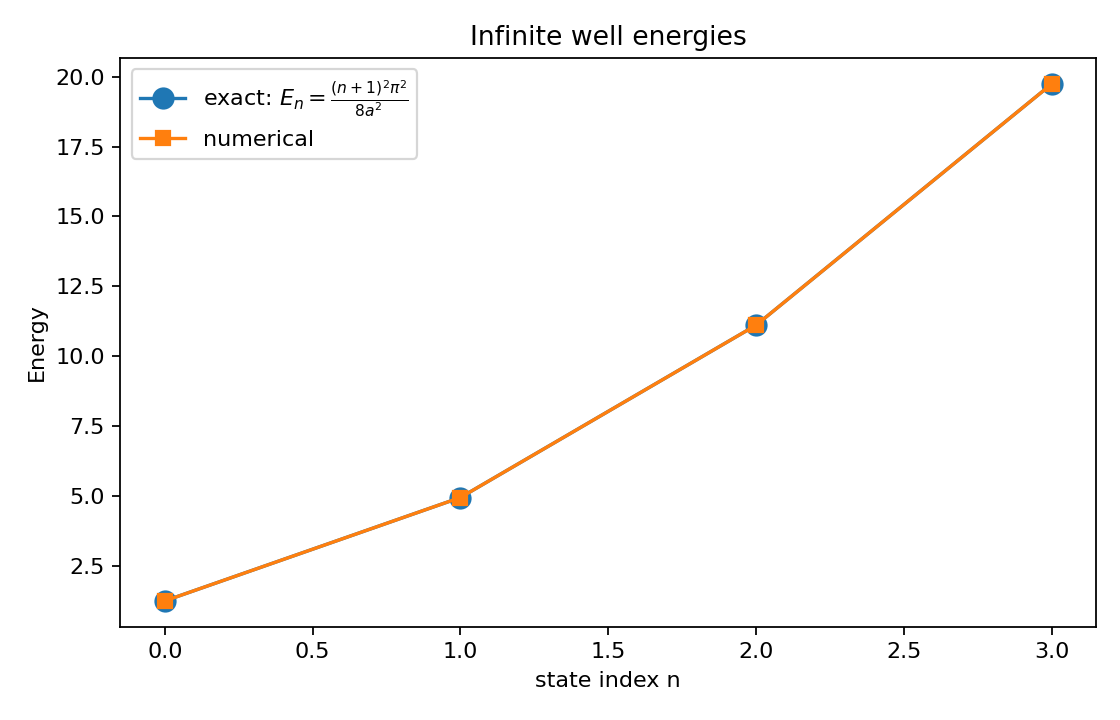
\includegraphics[height=5cm]{../results/1_infinite_square_well_Numerov/1_infinite_square_well_Numerov_energy_comparison.png}
                \caption{Comparison between numerical and exact energy eigenvalues for the infinite square well. The agreement is excellent for the first four states.}
                \label{fig:infwell_energies}
            \end{figure}

            \begin{figure}[!p]
                \centering
                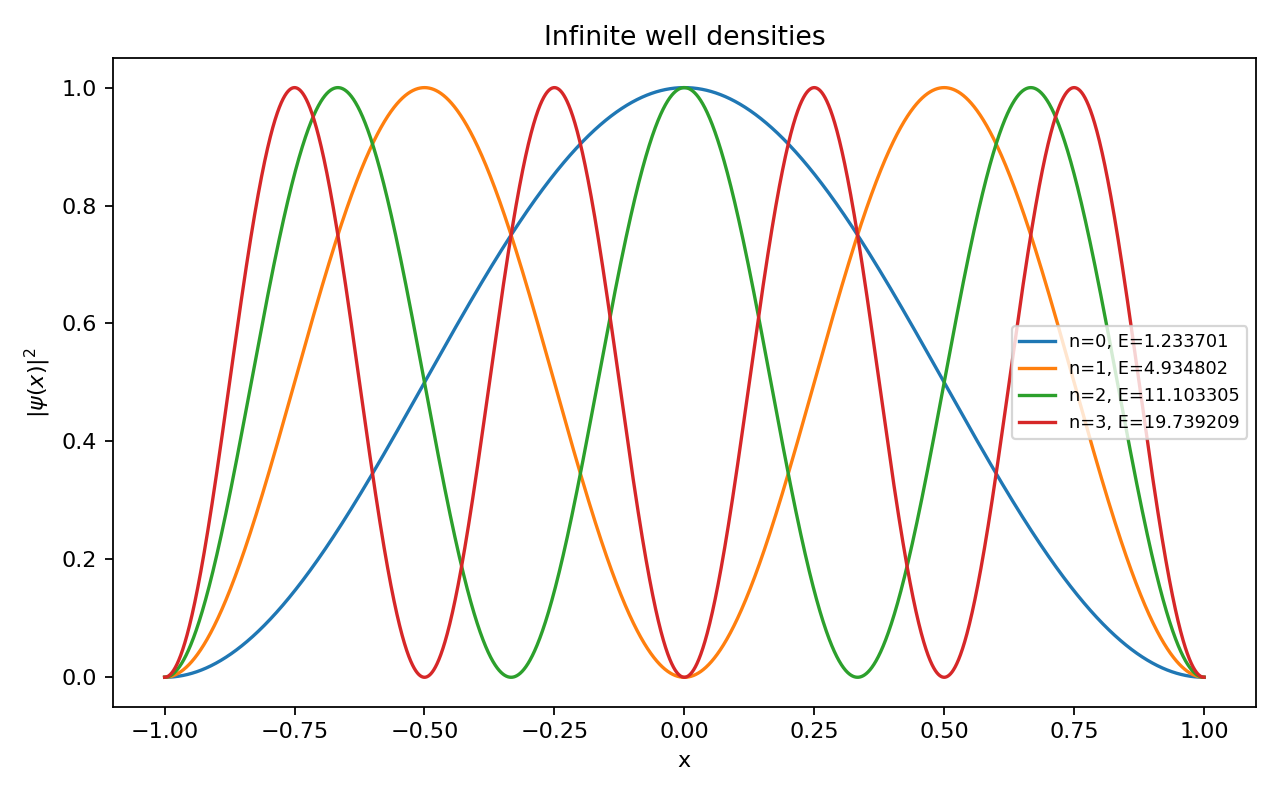
\includegraphics[height=5cm]{../results/1_infinite_square_well_Numerov/1_infinite_square_well_Numerov_densities.png}
                \caption{Probability densities $|\psi(x)|^2$ for the first four eigenstates of the infinite square well. The correct number of nodes and boundary behavior are clearly reproduced.}
                \label{fig:infwell_densities}
            \end{figure}

            \begin{figure}[!p]
                \centering
                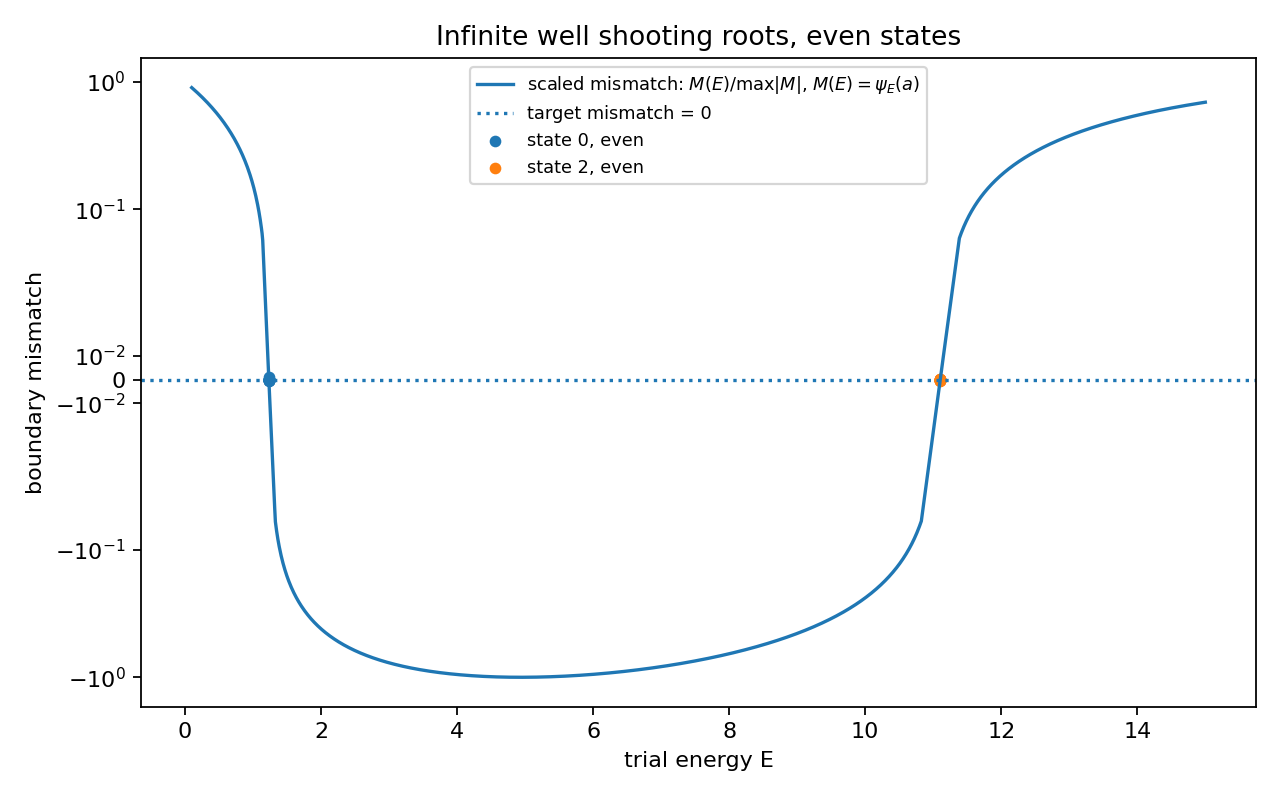
\includegraphics[height=5cm]{../results/1_infinite_square_well_Numerov/1_infinite_square_well_Numerov_root_finding_even.png}
                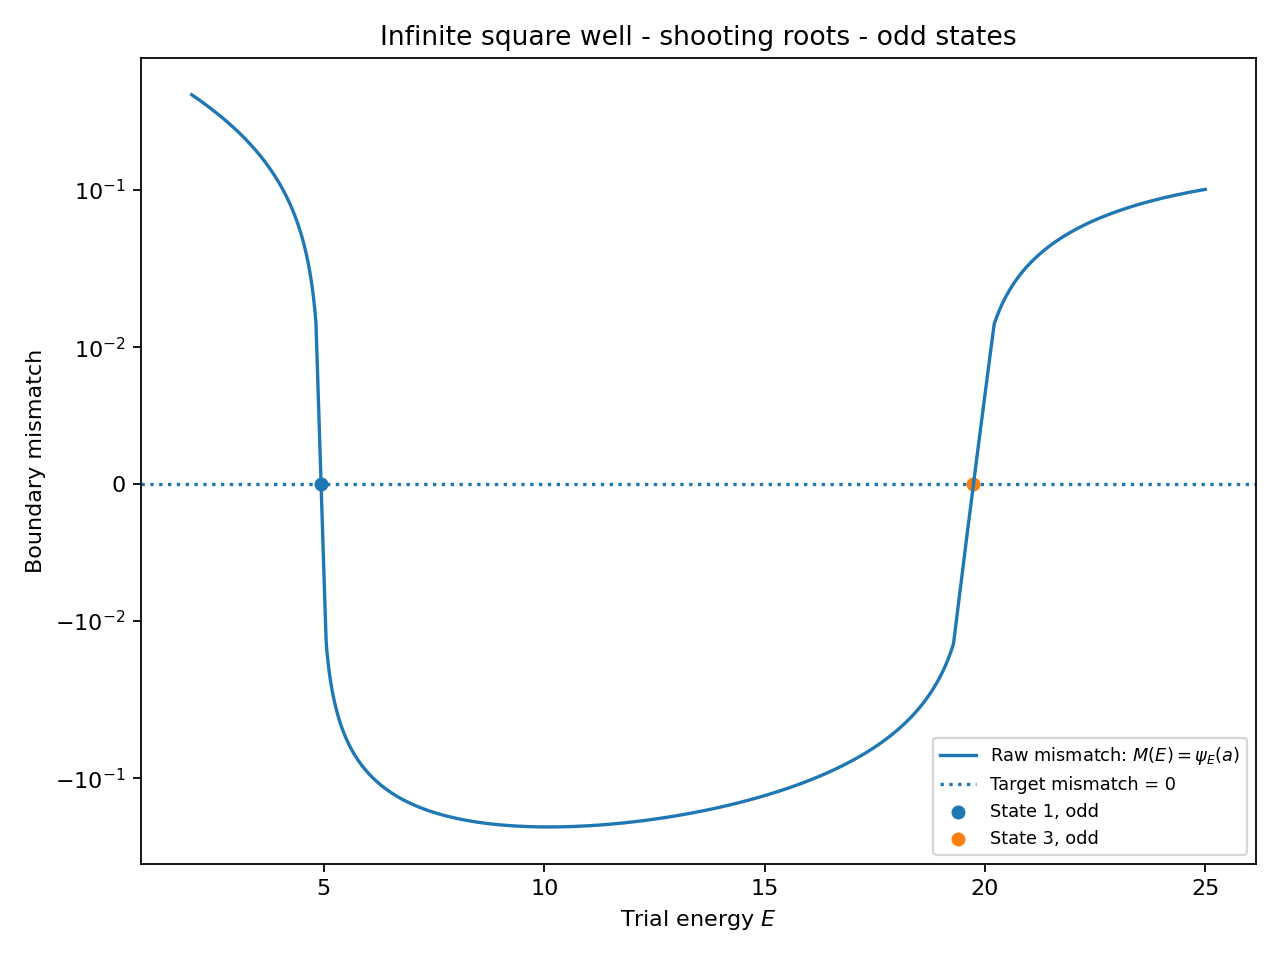
\includegraphics[height=5cm]{../results/1_infinite_square_well_Numerov/1_infinite_square_well_Numerov_root_finding_odd.png}
                \caption{Boundary mismatch functions for even (top) and odd (bottom) states. The zero crossings correspond to the physical eigenvalues found by the shooting method.}
                \label{fig:infwell_shooting}
            \end{figure}

            \begin{figure}[!p]
                \centering
                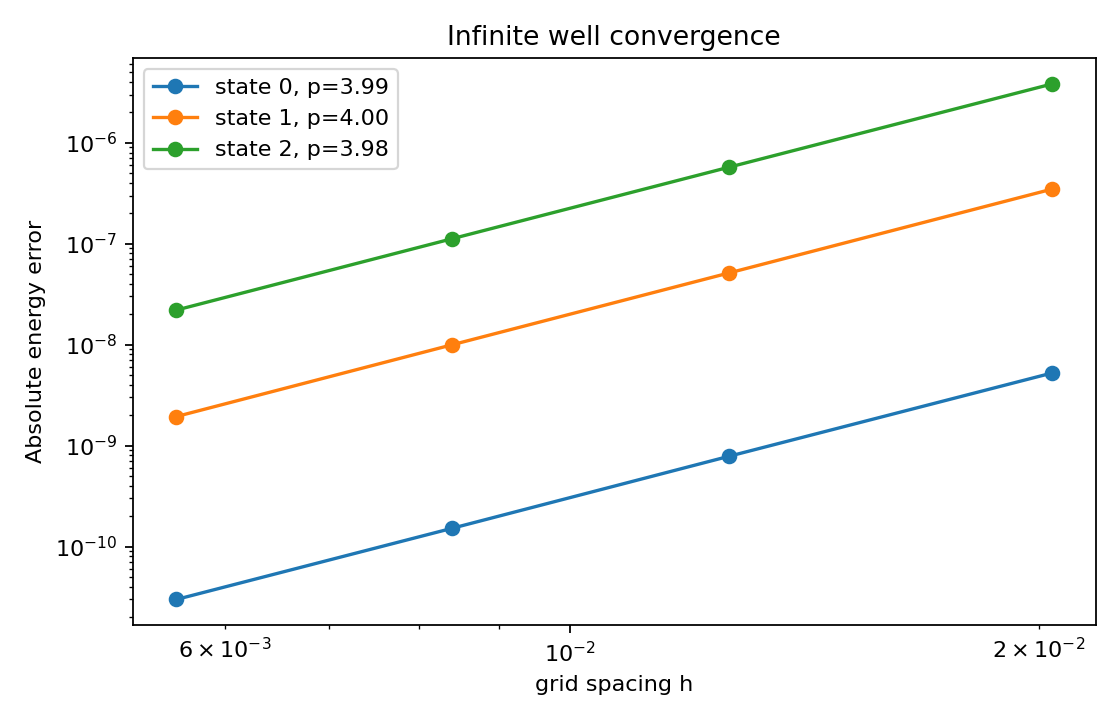
\includegraphics[height=5cm]{../results/1_infinite_square_well_Numerov/1_infinite_square_well_Numerov_convergence_vs_h.png}
                \caption{Convergence of the energy error as a function of grid spacing $h$. The slopes are close to fourth order, as expected for the Numerov method.}
                \label{fig:infwell_convergence}
            \end{figure}

            \begin{figure}[!p]
                \centering
                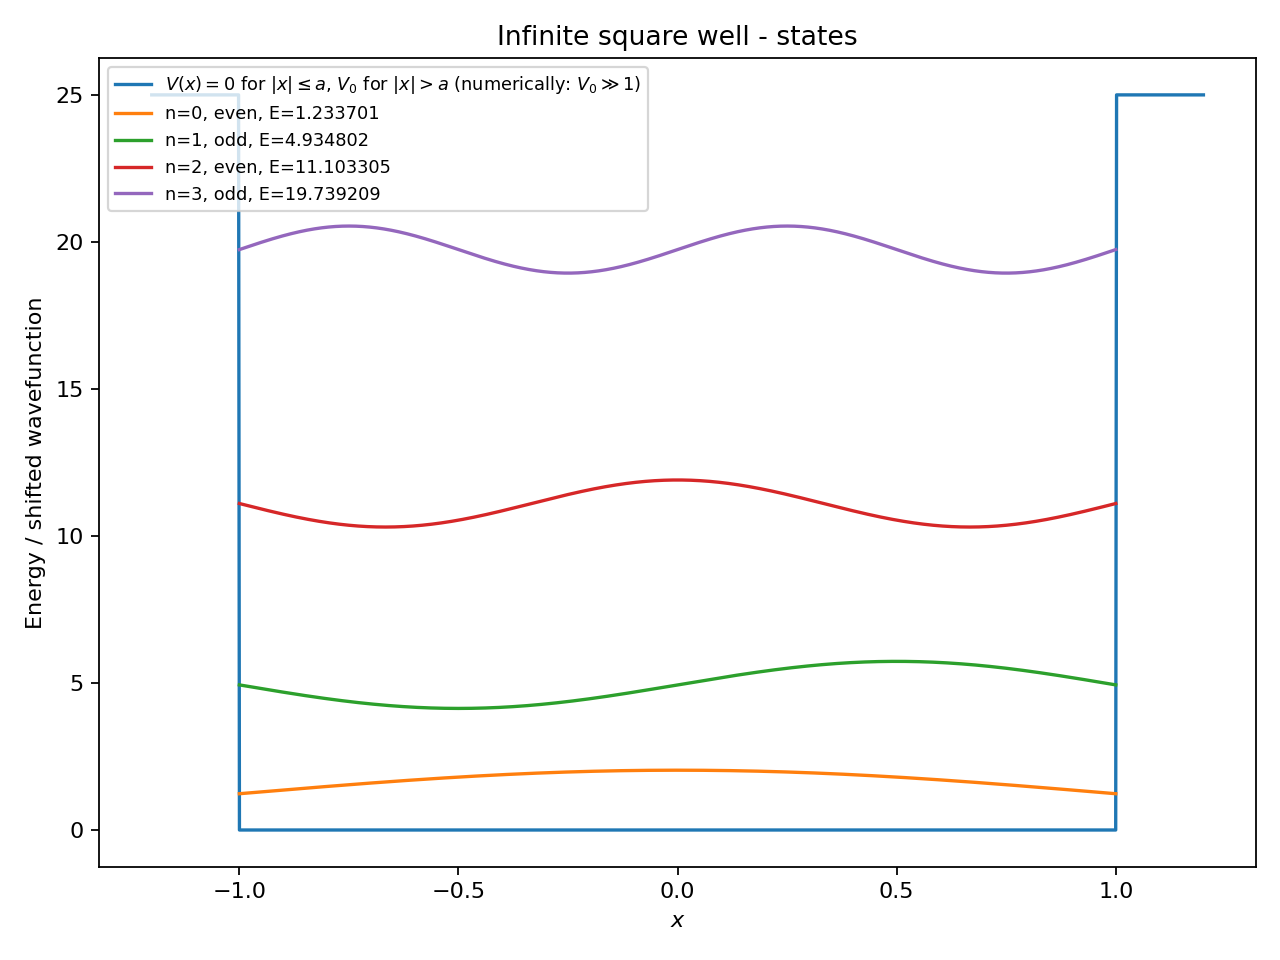
\includegraphics[height=5cm]{../results/1_infinite_square_well_Numerov/1_infinite_square_well_Numerov_states.png}
                \caption{Wavefunctions for the first four states plotted together with their corresponding energies and the confining potential.}
                \label{fig:infwell_states}
            \end{figure}

        \subsection{Harmonic oscillator}
            \subsubsection{Numerov method on unbounded domains}
                For the harmonic oscillator with $V(x)=\tfrac{1}{2}\omega^2 x^2$, the exact spectrum is
                \[
                E_n = \omega\left(n+\tfrac{1}{2}\right), \qquad n=0,1,2,\ldots
                \]
                This provides a second analytic benchmark, but on an unbounded domain. Numerically, the domain is truncated to $[-x_{\max},x_{\max}]$, and decaying boundary conditions are imposed.

                The numerical eigenvalues agree with the exact linear spectrum to high precision, as shown in Fig.~\ref{fig:ho_energies}. This confirms that the inward-shooting formulation correctly handles the exponentially decaying asymptotic behavior.

                The probability densities (Fig.~\ref{fig:ho_densities}) show the expected structure: the ground state is Gaussian-like with no nodes, while higher states exhibit the correct number of nodes and increasing spatial extent. This confirms both physical correctness and stability of the integration on a truncated domain.

                The shooting mismatch functions (Fig.~\ref{fig:ho_shooting}) exhibit clear zero crossings at the eigenvalues. Even and odd states are separated using parity conditions at the origin, and the roots alternate as expected. Although the mismatch spans many orders of magnitude due to exponential behavior, the crossings remain well-defined, indicating a robust root-finding procedure.

                Convergence with respect to grid spacing $h$ (Fig.~\ref{fig:ho_convergence_h}) shows near fourth-order behavior for most states, consistent with the Numerov method. Slight deviations (e.g. $p>4$ for the ground state) are attributed to fitting in a regime close to machine precision rather than a true increase in order.

                The dependence on domain size (Fig.~\ref{fig:ho_convergence_xmax}) shows rapid error reduction as $x_{\max}$ increases, followed by a plateau. This reflects the transition from truncation error (small $x_{\max}$) to discretization and floating-point limits (large $x_{\max}$).

                Finally, the combined state plot (Fig.~\ref{fig:ho_states}) shows the wavefunctions together with the confining potential. The spatial extent increases with energy, and the states remain well-behaved across the domain.

                \begin{figure}[!p]
                    \centering
                    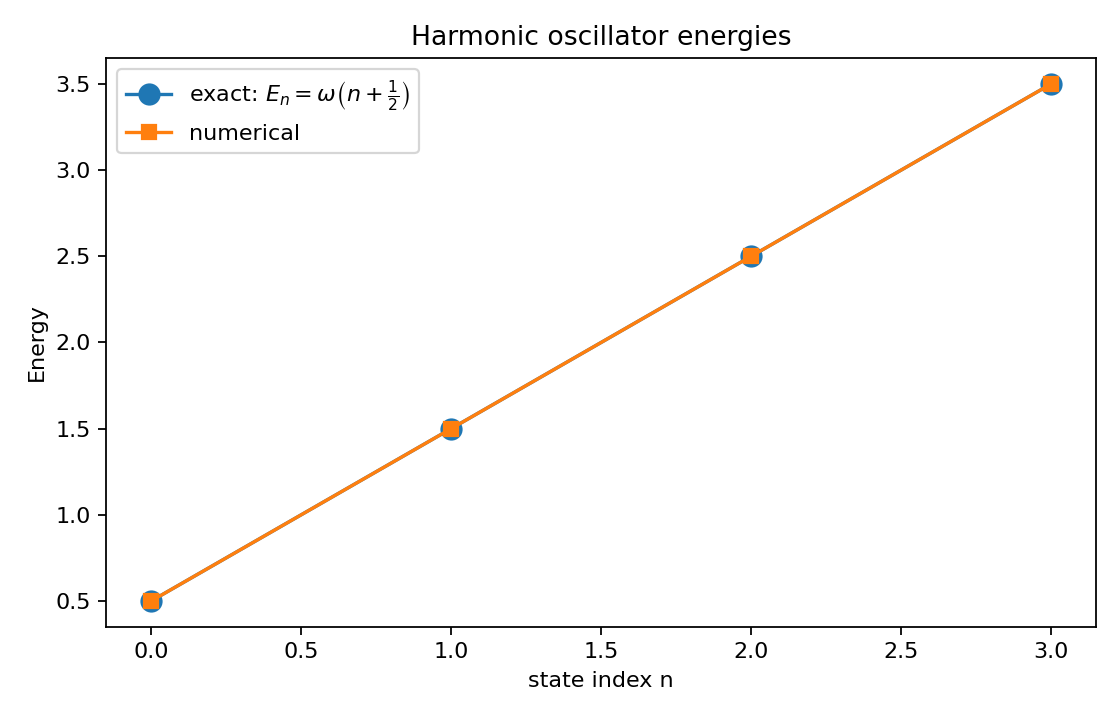
\includegraphics[height=5cm]{../results/2a_harmonic_oscillator_Numerov/2a_harmonic_oscillator_Numerov_energy_comparison.png}
                    \caption{Comparison between numerical and exact energy eigenvalues for the harmonic oscillator. The agreement is excellent for the first four states.}
                    \label{fig:ho_energies}
                \end{figure}

                \begin{figure}[!p]
                    \centering
                    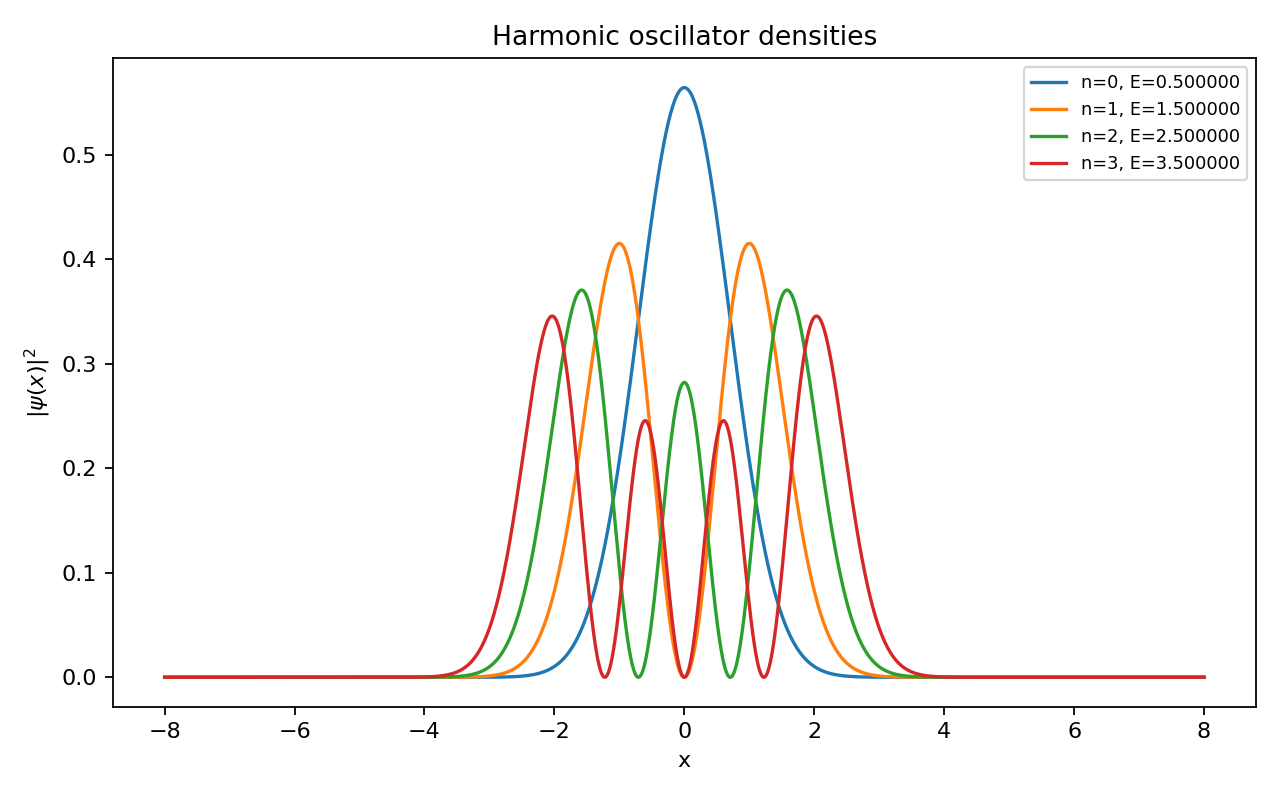
\includegraphics[height=5cm]{../results/2a_harmonic_oscillator_Numerov/2a_harmonic_oscillator_Numerov_densities.png}
                    \caption{Probability densities $|\psi(x)|^2$ for the first four harmonic oscillator eigenstates. The correct node structure is clearly reproduced.}
                    \label{fig:ho_densities}
                \end{figure}

                \begin{figure}[!p]
                    \centering
                    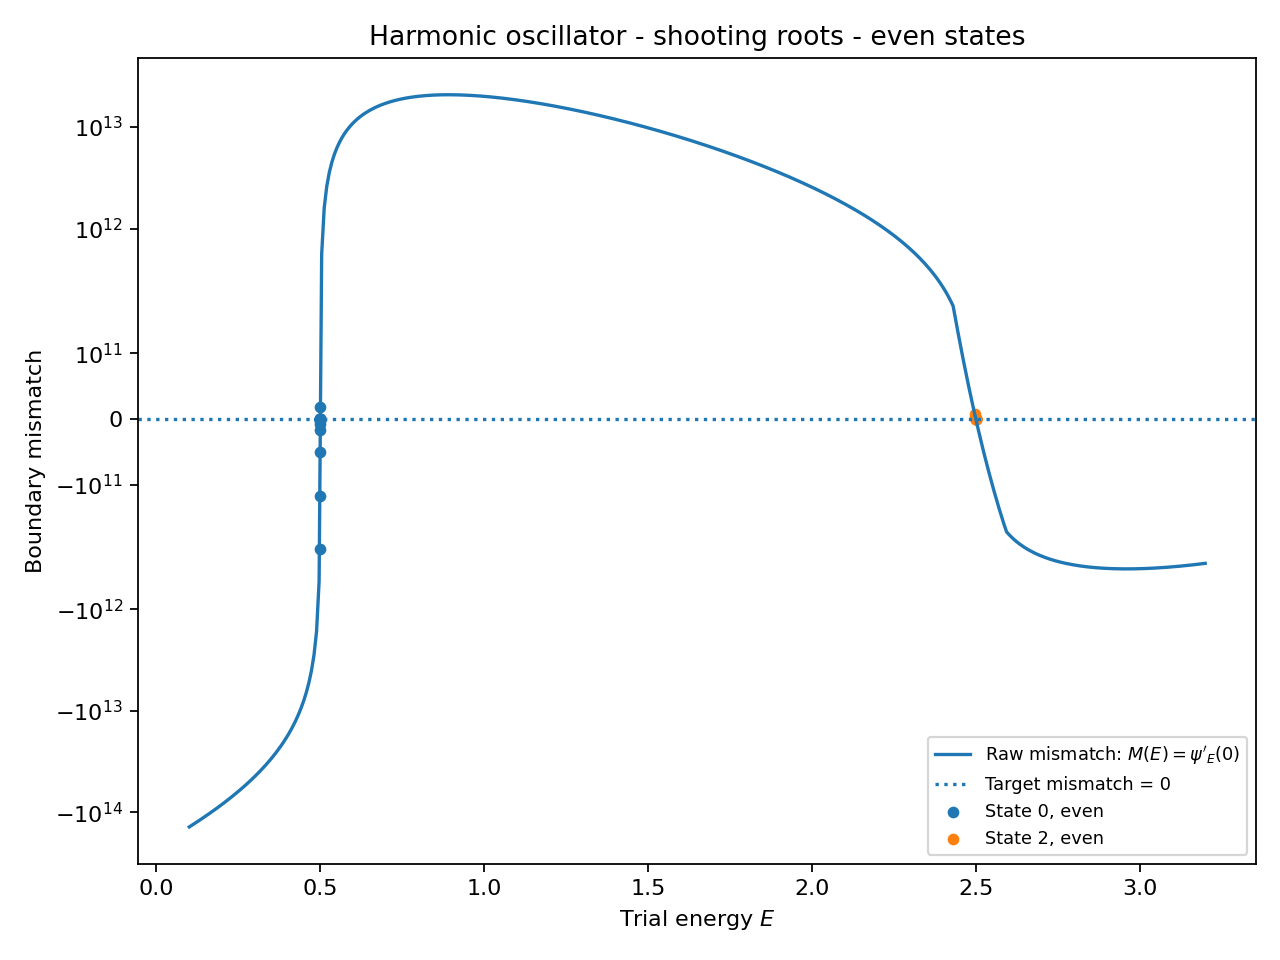
\includegraphics[height=5cm]{../results/2a_harmonic_oscillator_Numerov/2a_harmonic_oscillator_Numerov_root_finding_even.png}
                    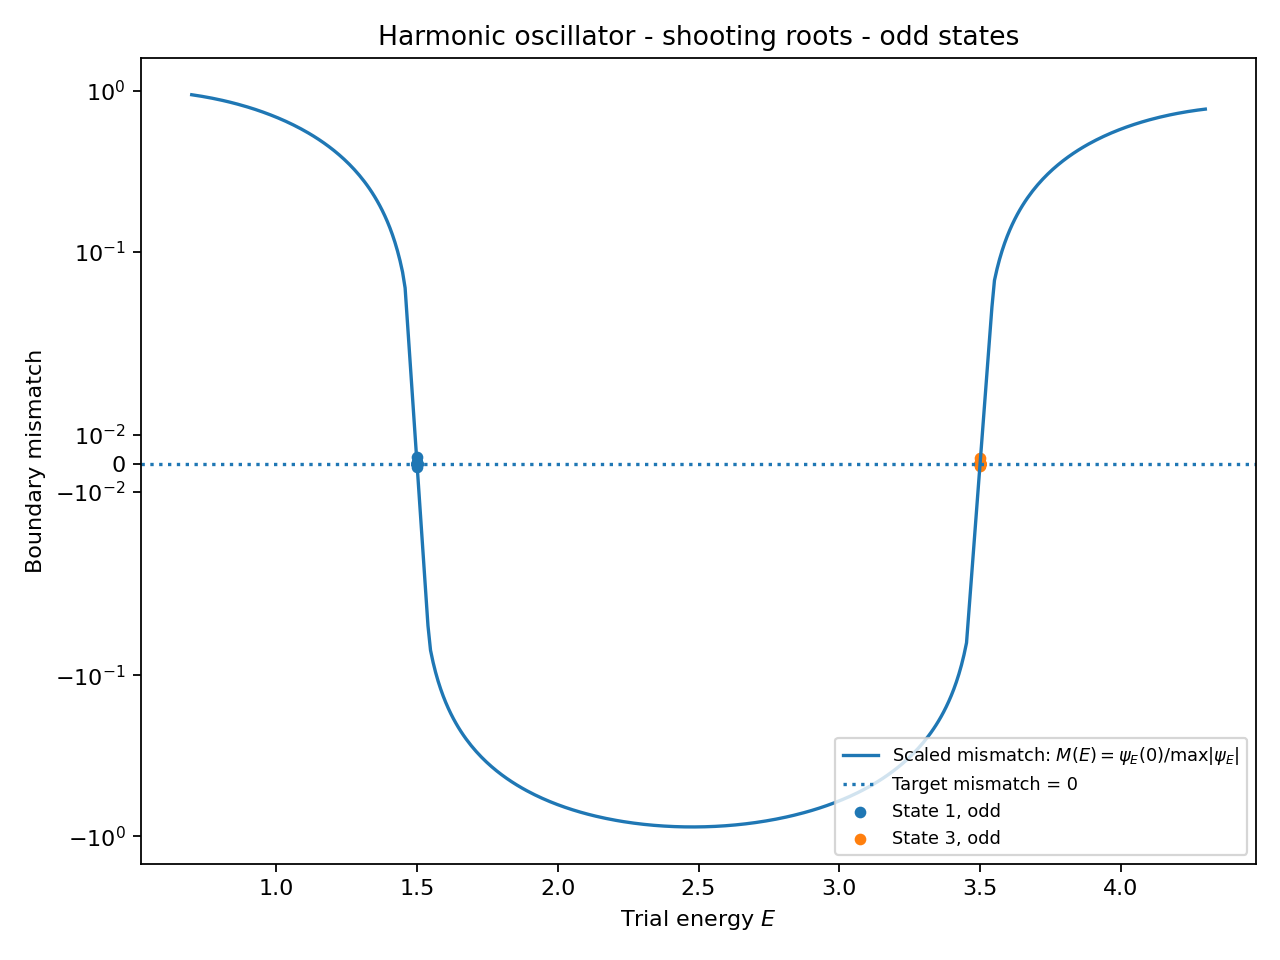
\includegraphics[height=5cm]{../results/2a_harmonic_oscillator_Numerov/2a_harmonic_oscillator_Numerov_root_finding_odd.png}
                    \caption{Boundary mismatch functions for even (top) and odd (bottom) states. The zero crossings correspond to the physical eigenvalues.}
                    \label{fig:ho_shooting}
                \end{figure}

                \begin{figure}[!p]
                    \centering
                    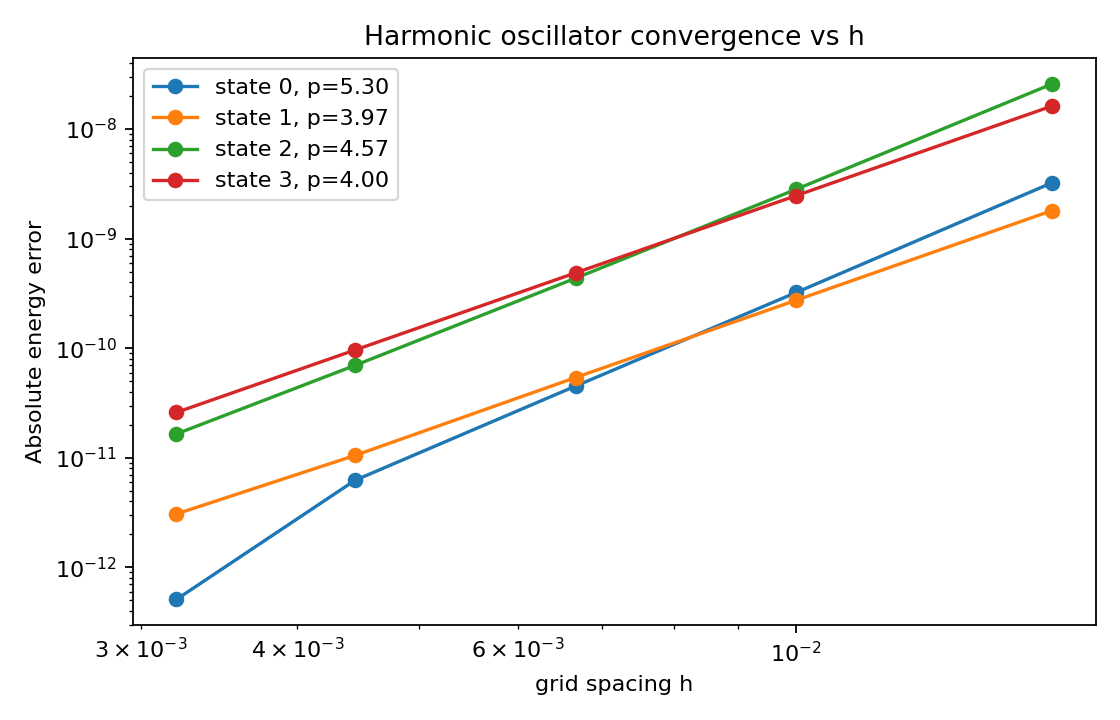
\includegraphics[height=5cm]{../results/2a_harmonic_oscillator_Numerov/2a_harmonic_oscillator_Numerov_convergence_vs_h.png}
                    \caption{Convergence of the energy error as a function of grid spacing $h$. The slopes are close to fourth order, as expected for the Numerov method.}
                    \label{fig:ho_convergence_h}
                \end{figure}

                \begin{figure}[!p]
                    \centering
                    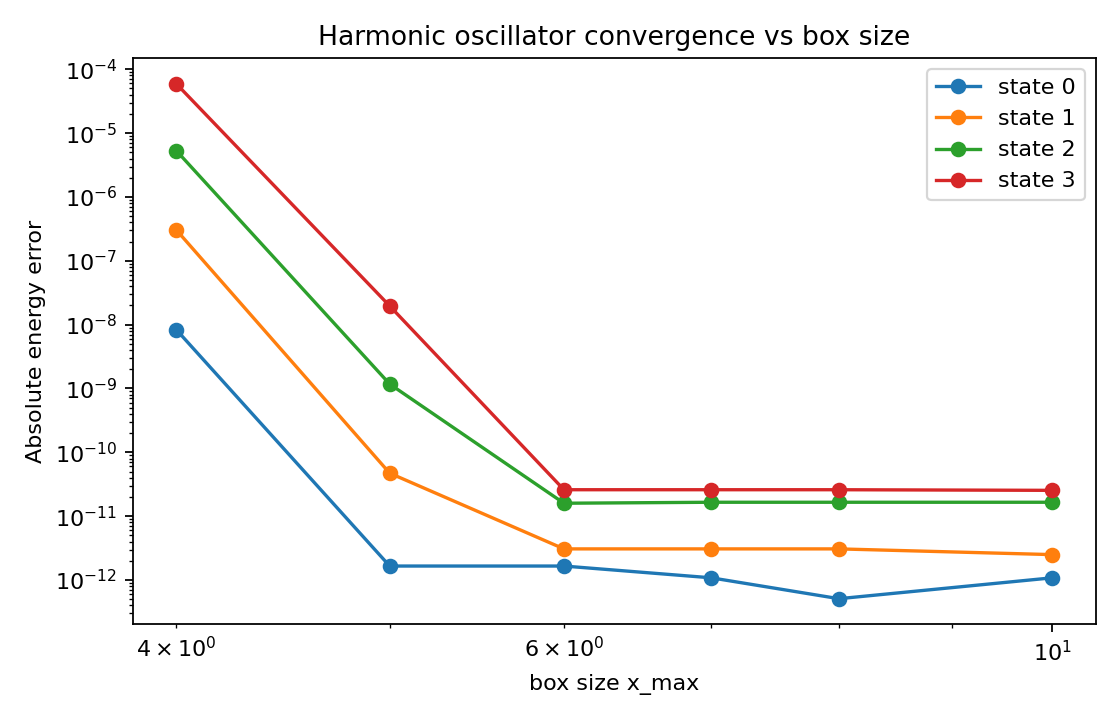
\includegraphics[height=5cm]{../results/2a_harmonic_oscillator_Numerov/2a_harmonic_oscillator_Numerov_convergence_vs_x_max.png}
                    \caption{Dependence of the energy error on the domain size $x_{\max}$. Errors decrease rapidly before reaching a plateau set by discretization and floating-point limits.}
                    \label{fig:ho_convergence_xmax}
                \end{figure}

                \begin{figure}[!p]
                    \centering
                    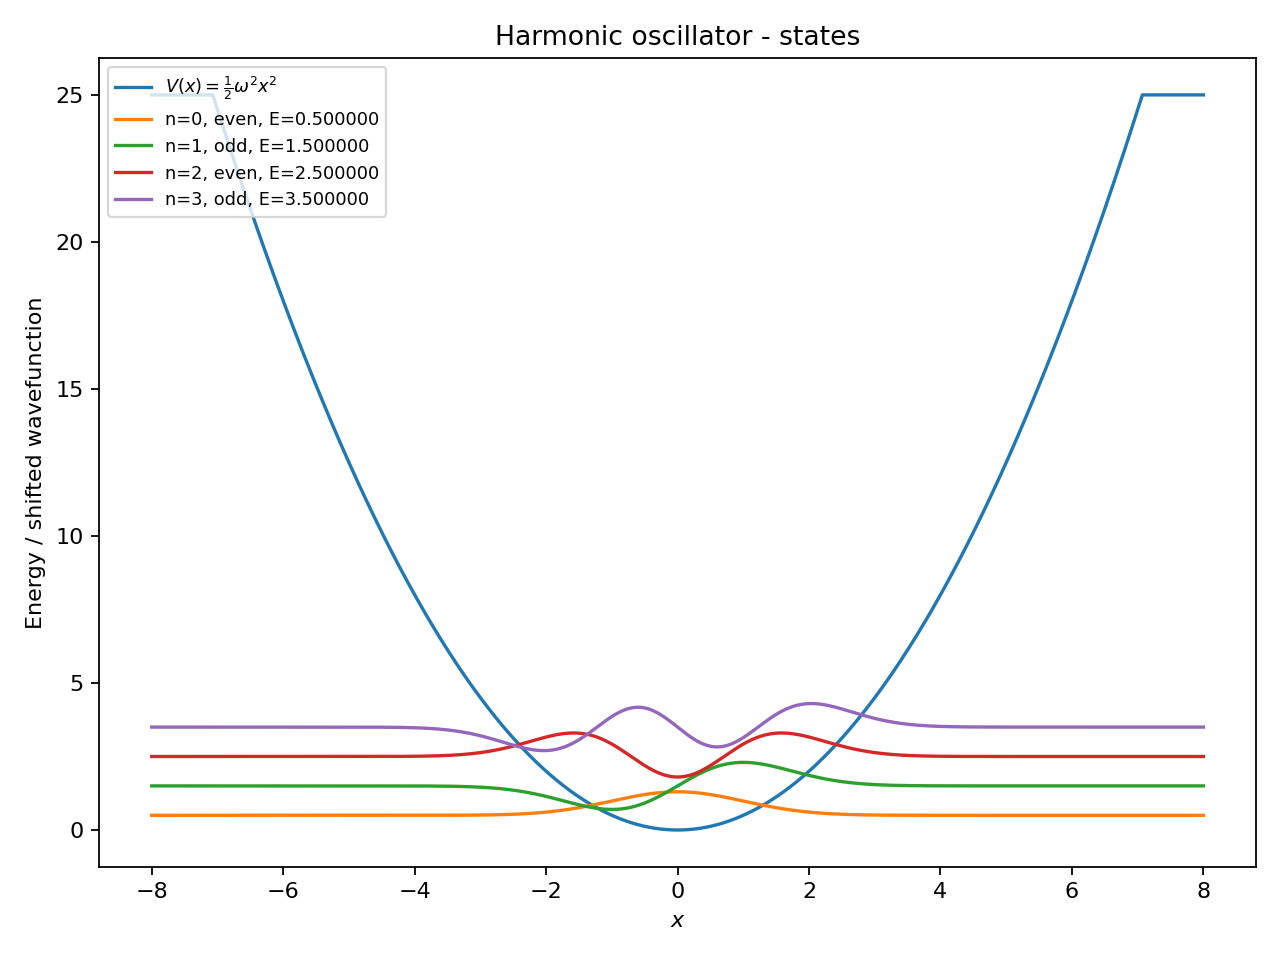
\includegraphics[height=5cm]{../results/2a_harmonic_oscillator_Numerov/2a_harmonic_oscillator_Numerov_states.png}
                    \caption{Wavefunctions for the first four harmonic oscillator states plotted together with the potential.}
                    \label{fig:ho_states}
                \end{figure}

            \subsubsection{Numerov versus Runge--Kutta}
                As an additional method comparison, the harmonic oscillator was also solved using a fourth-order Runge--Kutta (RK4) shooting method. In this formulation the second-order Schr\"odinger equation is rewritten as the first-order system
                \[
                \psi' = \phi, \qquad
                \phi' = 2[V(x)-E]\psi .
                \]
                This makes RK4 a useful general-purpose comparison for Numerov, which instead exploits the special second-order structure of the Schr\"odinger equation directly.

                Figure~\ref{fig:ho_numerov_vs_rk4} compares the maximum energy error over the computed harmonic-oscillator states as a function of grid spacing. Both methods show approximately fourth-order convergence, as expected. Numerov is consistently more accurate for the same grid spacing, although the difference is moderate. This is consistent with the fact that both methods are already high-order and that the final accuracy is also affected by root-finding tolerance, domain truncation, and boundary-condition treatment.

                This comparison also emphasizes an important numerical point: the order of the integration scheme alone is not sufficient. Boundary conditions and diagnostic quantities must be evaluated with comparable accuracy. After using a high-order boundary derivative for the Numerov inward-shooting condition, the Numerov and RK4 comparison behaves as expected.

                \begin{figure}[!p]
                    \centering
                    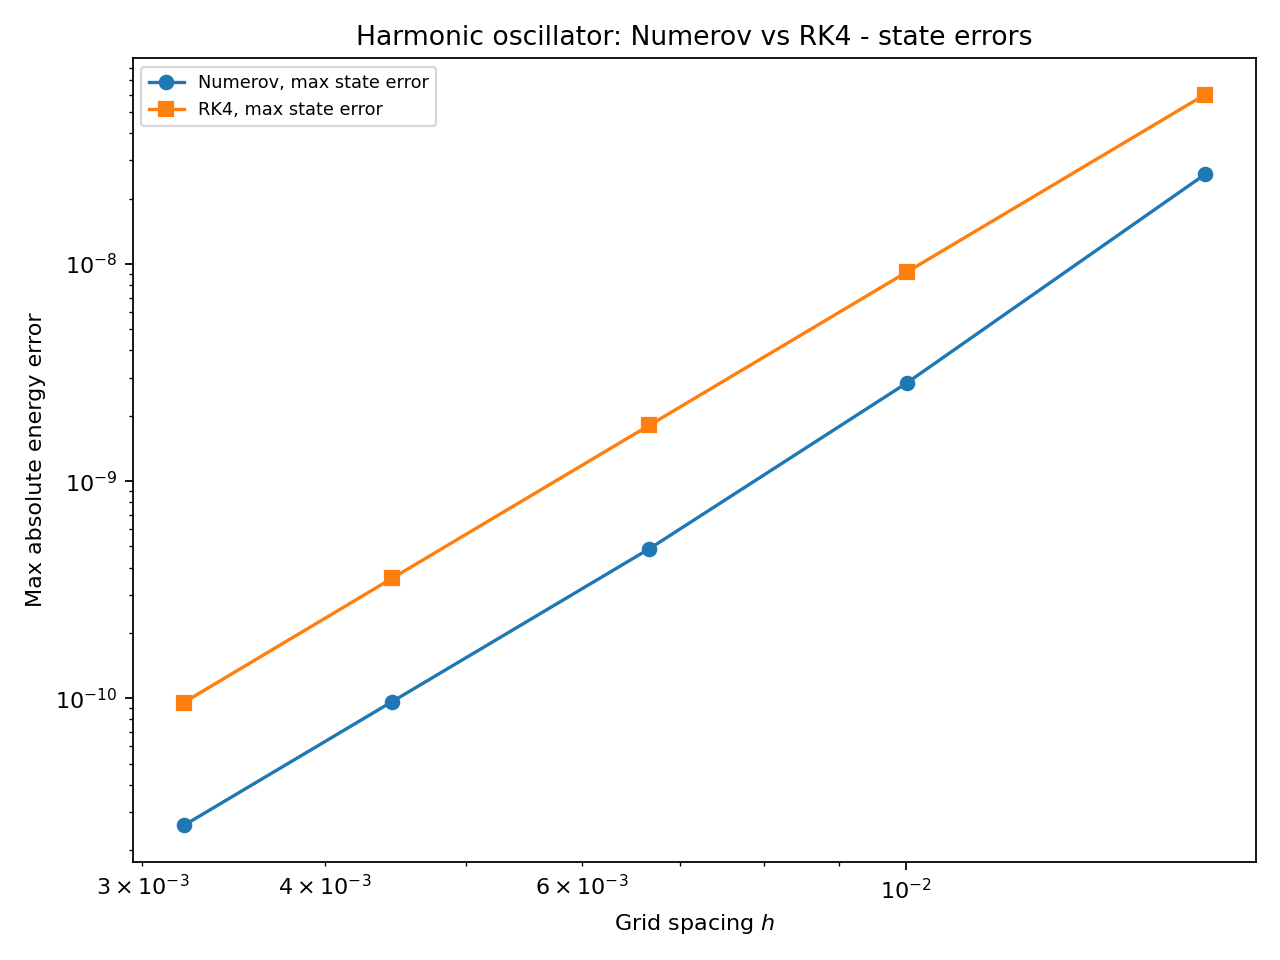
\includegraphics[height=5cm]{../results/2c_harmonic_oscillator_Numerov_VS_RK4_comparison/2c_harmonic_numerov_vs_rk4.png}
                    \caption{Comparison of Numerov and RK4 shooting for the harmonic oscillator. Both methods show fourth-order convergence, while Numerov gives a smaller maximum energy error at the same grid spacing.}
                    \label{fig:ho_numerov_vs_rk4}
                \end{figure}

        \subsection{Double-well potential}
            The quartic double-well potential is used as the main nontrivial bound-state example. In the shifted form used here,
            \[
            V(x)=ax^4-bx^2-V_{\min}, \qquad V_{\min}=-\frac{b^2}{4a},
            \]
            the two minima are shifted to zero. Unlike the infinite square well and harmonic oscillator, this system does not have a simple analytic spectrum, so the validation relies on internal consistency checks, convergence studies, parity structure, and physically expected tunneling behavior.

            Figure~\ref{fig:dw_states} shows the first four computed states together with the double-well potential. The two lowest states form a nearly degenerate even-odd pair, with energies $E_0\approx2.357273$ and $E_1\approx2.359372$. This is the expected tunneling doublet: the even and odd states are symmetric and antisymmetric combinations of states localized in the two wells. The next pair is higher in energy and has a larger splitting, consistent with stronger overlap through the barrier.

            The probability densities in Fig.~\ref{fig:dw_densities} show the expected localization near the two wells. The lowest pair has nearly identical density, because the sign difference between even and odd wavefunctions disappears in $|\psi(x)|^2$. The higher states show additional node structure and broader support, as expected for excited double-well states.

            The root-finding diagnostics (Fig.~\ref{fig:dw_shooting}) show well-defined zero crossings in the even and odd parity sectors. These plots verify that the computed energies are roots of the shooting mismatch function and that the parity separation continues to work for a more complicated potential.

            Since there is no closed-form exact spectrum for this potential, grid convergence is measured using successive refinements at fixed domain size. The convergence with respect to grid spacing (Fig.~\ref{fig:dw_convergence_h}) shows high-order behavior for the first four states, with fitted slopes close to or above fourth order. As in the harmonic oscillator case, slopes slightly above four should be interpreted as fitting artifacts in a very small-error regime, not as a true order higher than Numerov's expected order.

            The box-size study (Fig.~\ref{fig:dw_convergence_xmax}) shows rapid error reduction as the computational domain is enlarged, followed by a plateau near numerical precision. This confirms that the chosen domain is large enough for the bound states and that the final results are not dominated by artificial boundary truncation.

            Finally, Fig.~\ref{fig:dw_splitting} shows how the lowest even-odd splitting changes with the double-well parameter $b$. As $b$ increases, the barrier between the wells becomes more pronounced and the splitting decreases toward zero. This is the expected physical signature of tunneling suppression: increasing the barrier reduces overlap between the left- and right-localized components.

            Overall, the double-well results demonstrate that the solver works beyond analytic benchmarks. The computed states have the expected parity and localization, the tunneling splitting behaves physically, and the convergence studies show that the numerical results are stable with respect to both grid spacing and domain size.

            \begin{figure}[!p]
                \centering
                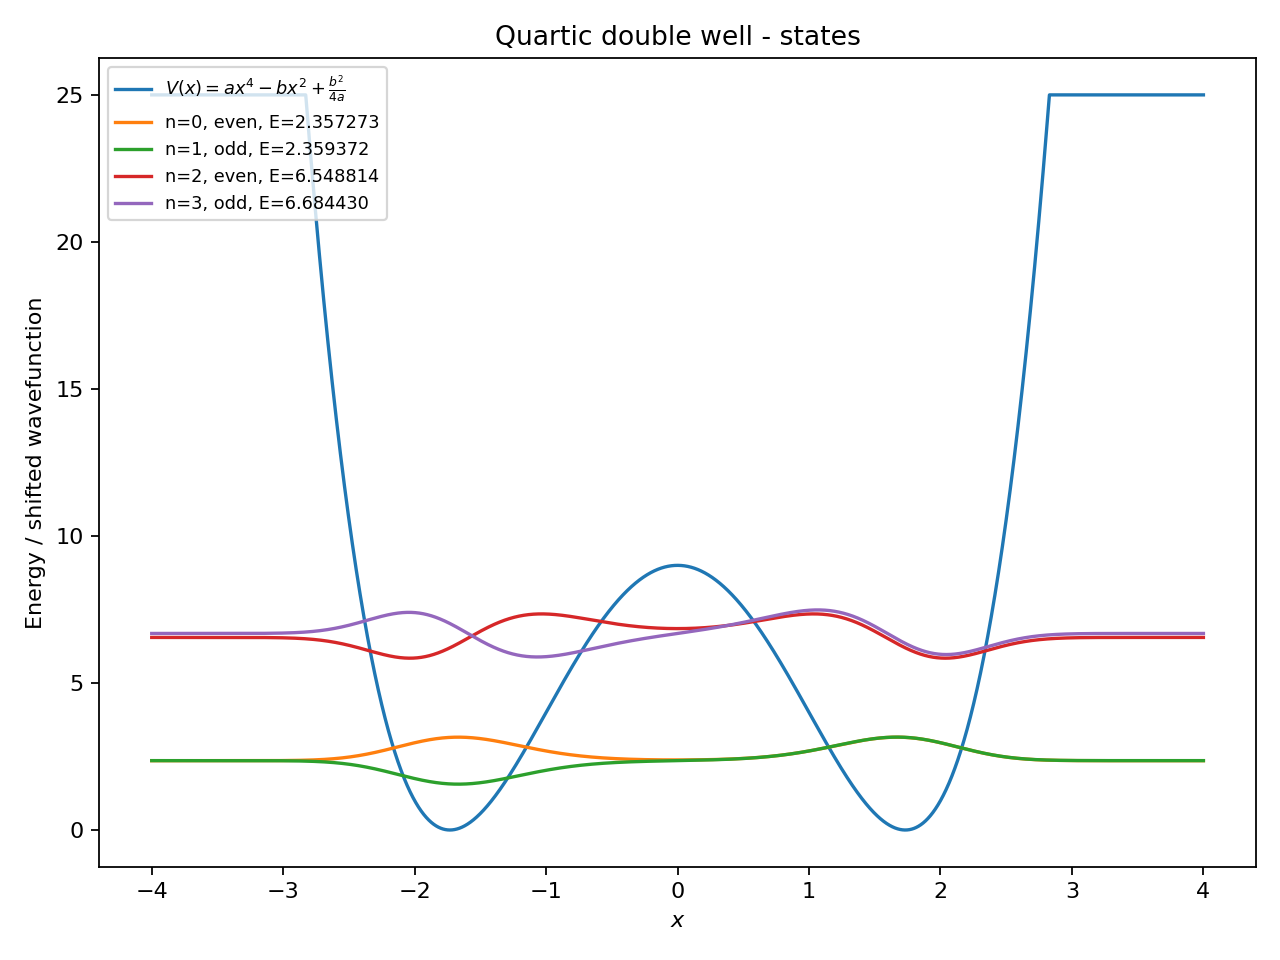
\includegraphics[height=5cm]{../results/3_double_well_Numerov/3_double_well_Numerov_states.png}
                \caption{First four bound states of the quartic double-well potential. The lowest two states form a nearly degenerate tunneling doublet.}
                \label{fig:dw_states}
            \end{figure}

            \begin{figure}[!p]
                \centering
                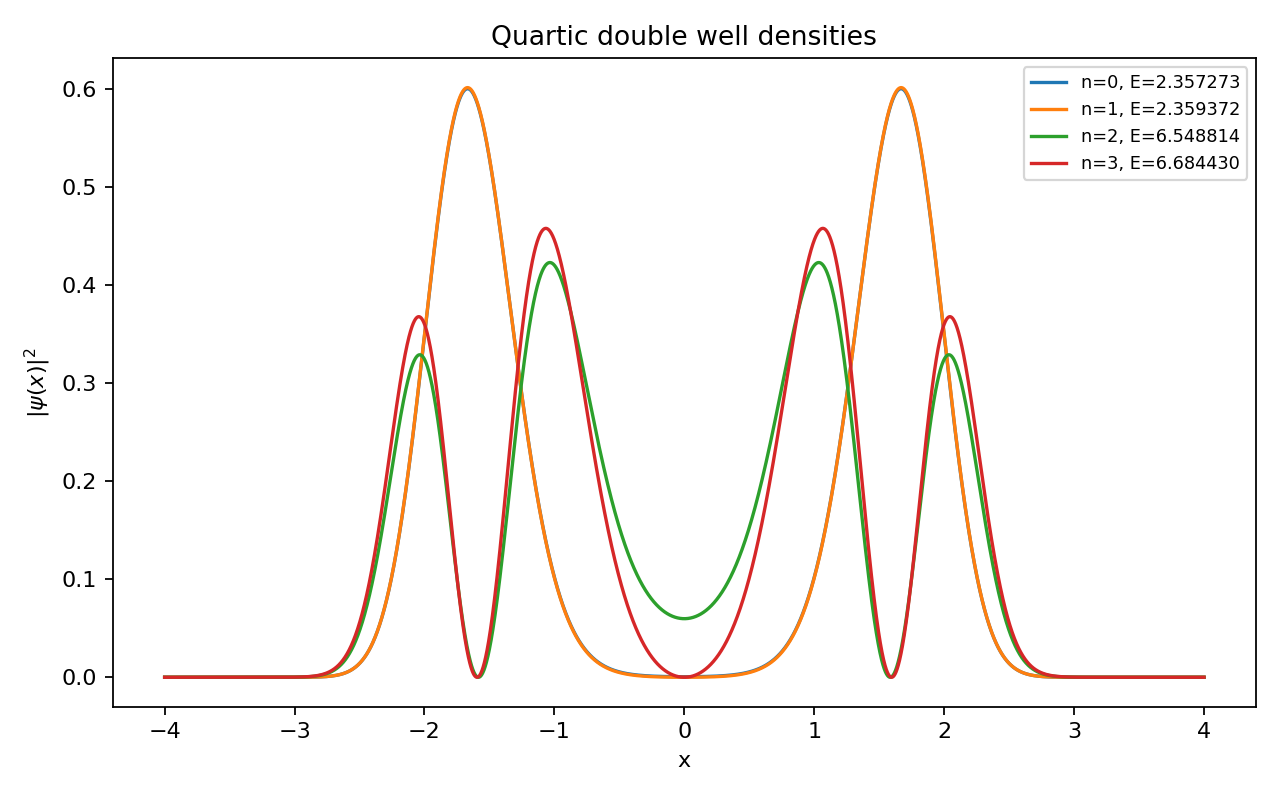
\includegraphics[height=5cm]{../results/3_double_well_Numerov/3_double_well_Numerov_densities.png}
                \caption{Probability densities $|\psi(x)|^2$ for the first four double-well states. The lowest even and odd states have nearly identical densities, as expected for a tunneling doublet.}
                \label{fig:dw_densities}
            \end{figure}

            \begin{figure}[!p]
                \centering
                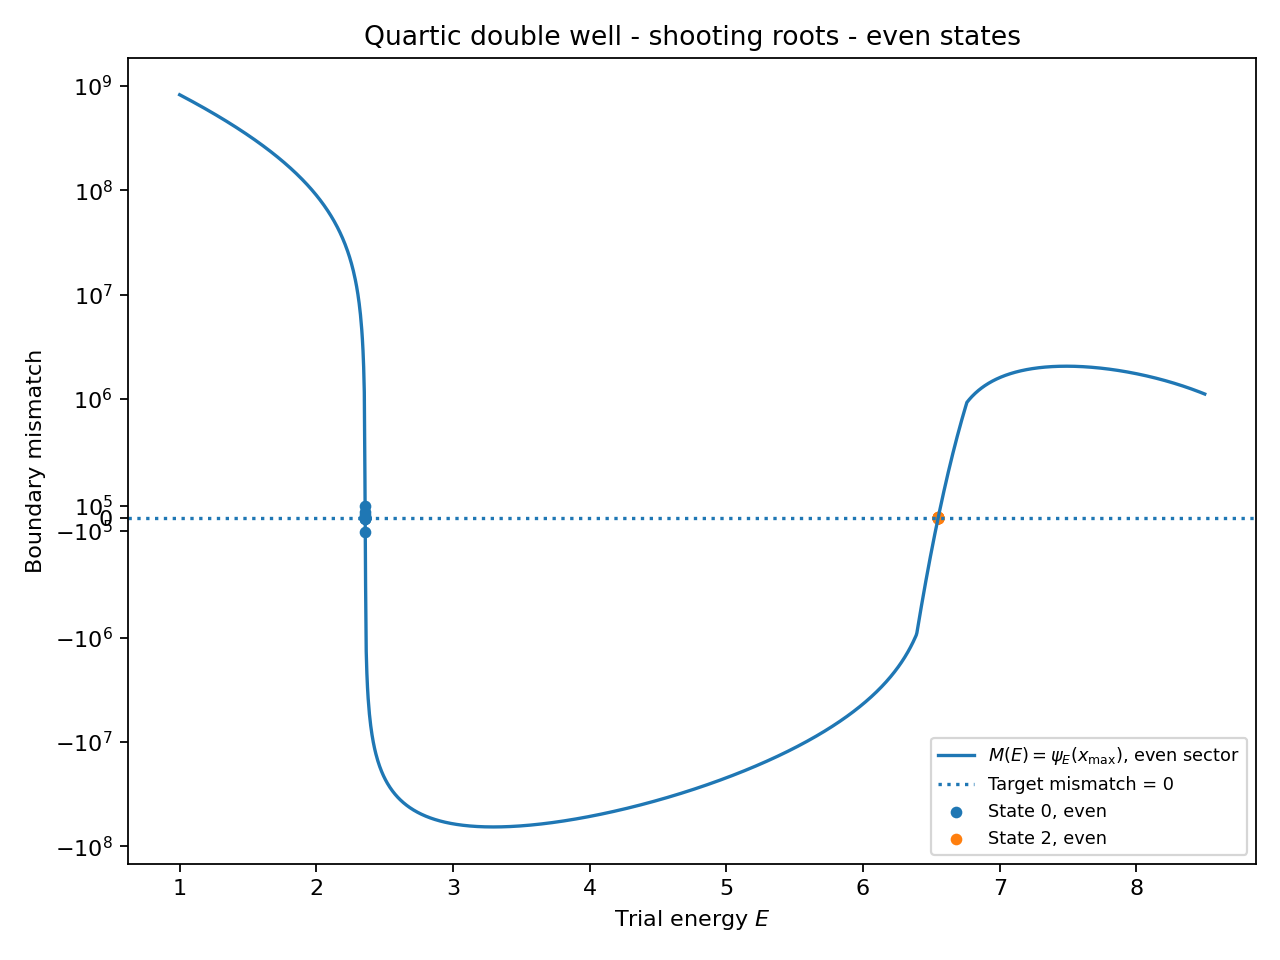
\includegraphics[height=5cm]{../results/3_double_well_Numerov/3_double_well_Numerov_root_finding_even.png}
                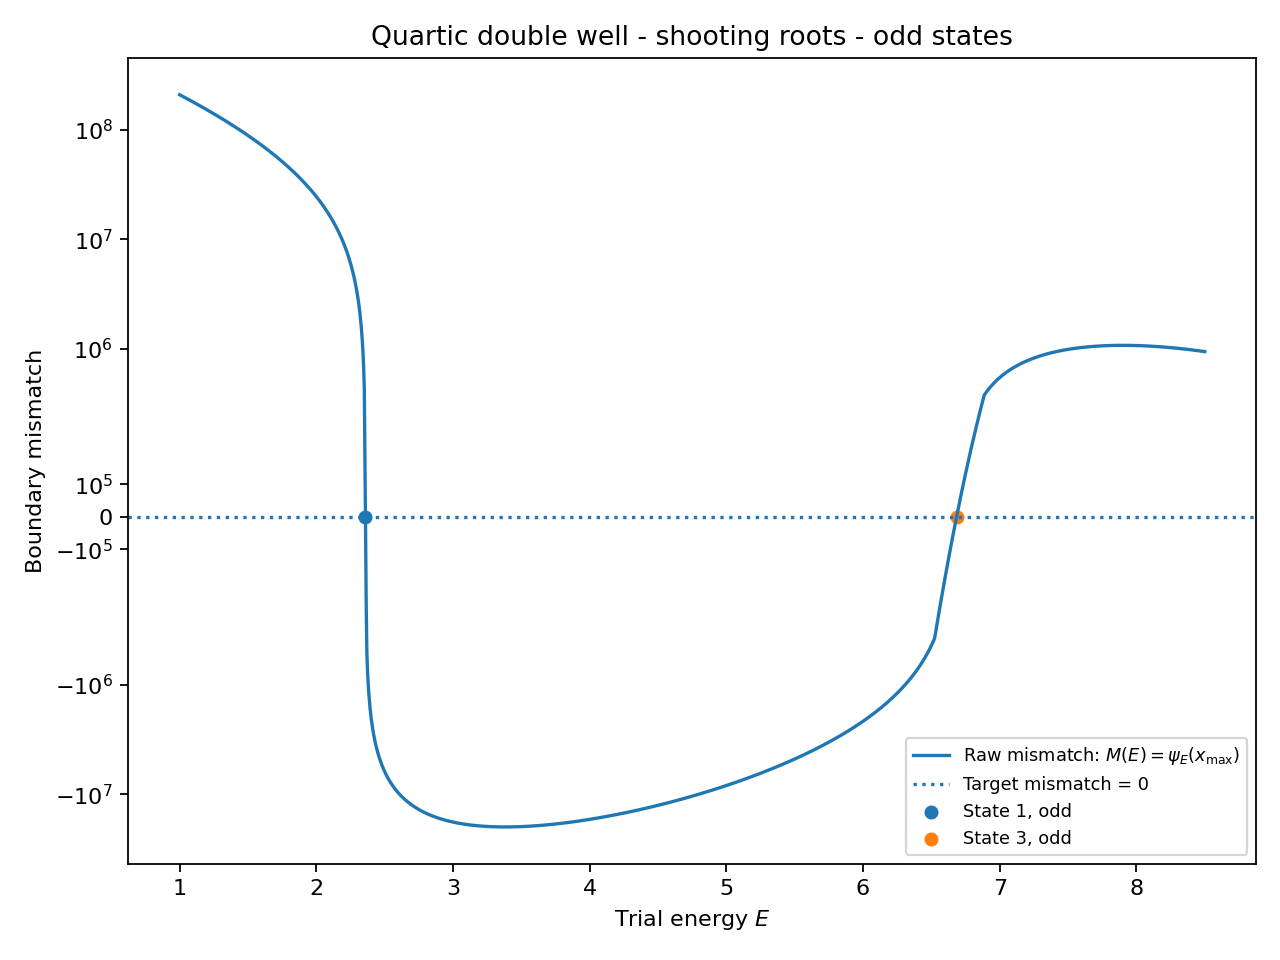
\includegraphics[height=5cm]{../results/3_double_well_Numerov/3_double_well_Numerov_root_finding_odd.png}
                \caption{Shooting mismatch functions for even (top) and odd (bottom) double-well states. The zero crossings define the numerical eigenvalues.}
                \label{fig:dw_shooting}
            \end{figure}

            \begin{figure}[!p]
                \centering
                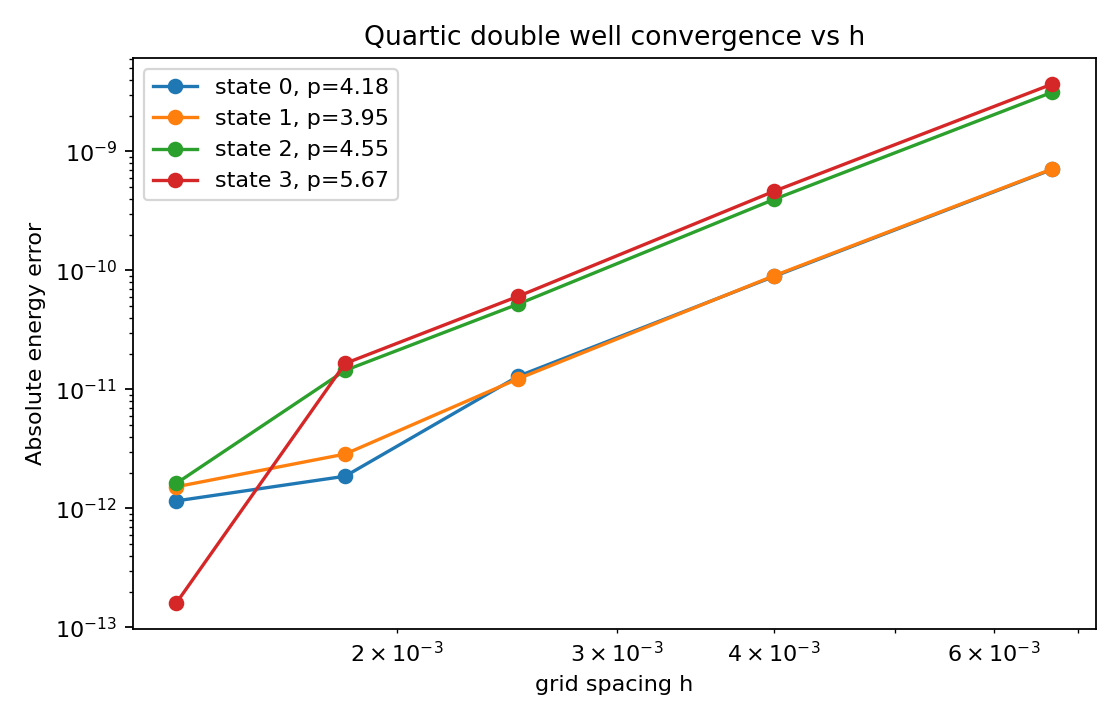
\includegraphics[height=5cm]{../results/3_double_well_Numerov/3_double_well_Numerov_convergence_vs_h.png}
                \caption{Grid convergence for the quartic double well. The energy errors decrease with high-order behavior under successive grid refinement.}
                \label{fig:dw_convergence_h}
            \end{figure}

            \begin{figure}[!p]
                \centering
                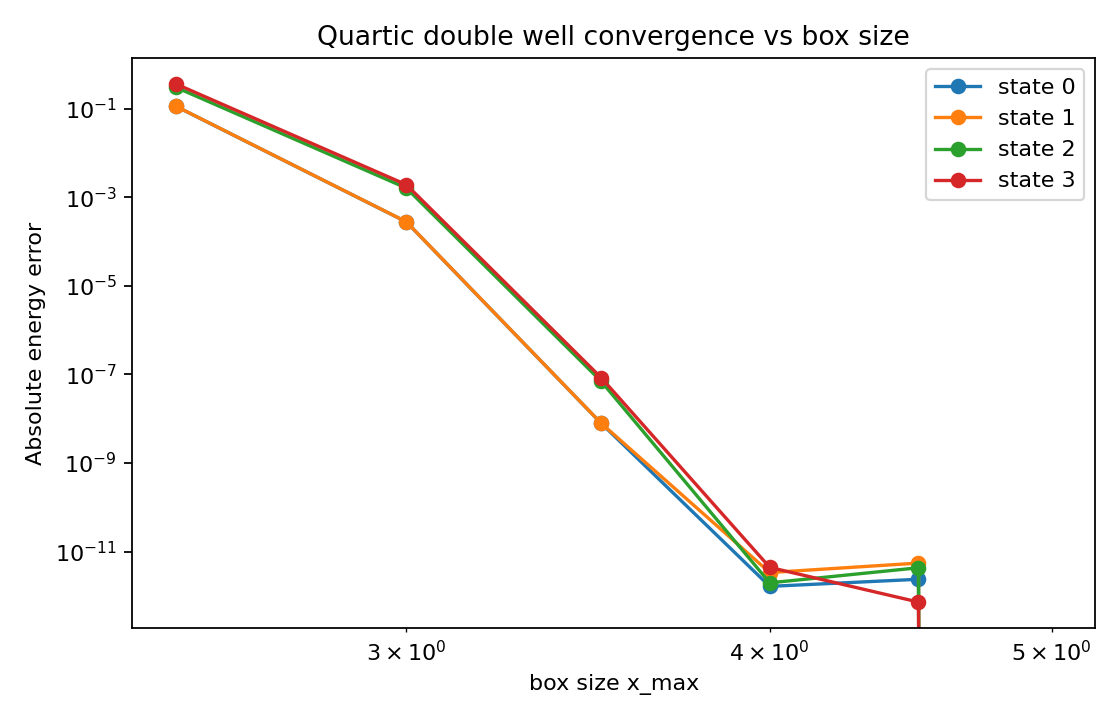
\includegraphics[height=5cm]{../results/3_double_well_Numerov/3_double_well_Numerov_convergence_vs_x_max.png}
                \caption{Dependence of the double-well energy errors on box size. The errors decrease rapidly as the domain is enlarged and then reach a numerical plateau.}
                \label{fig:dw_convergence_xmax}
            \end{figure}

            \begin{figure}[!p]
                \centering
                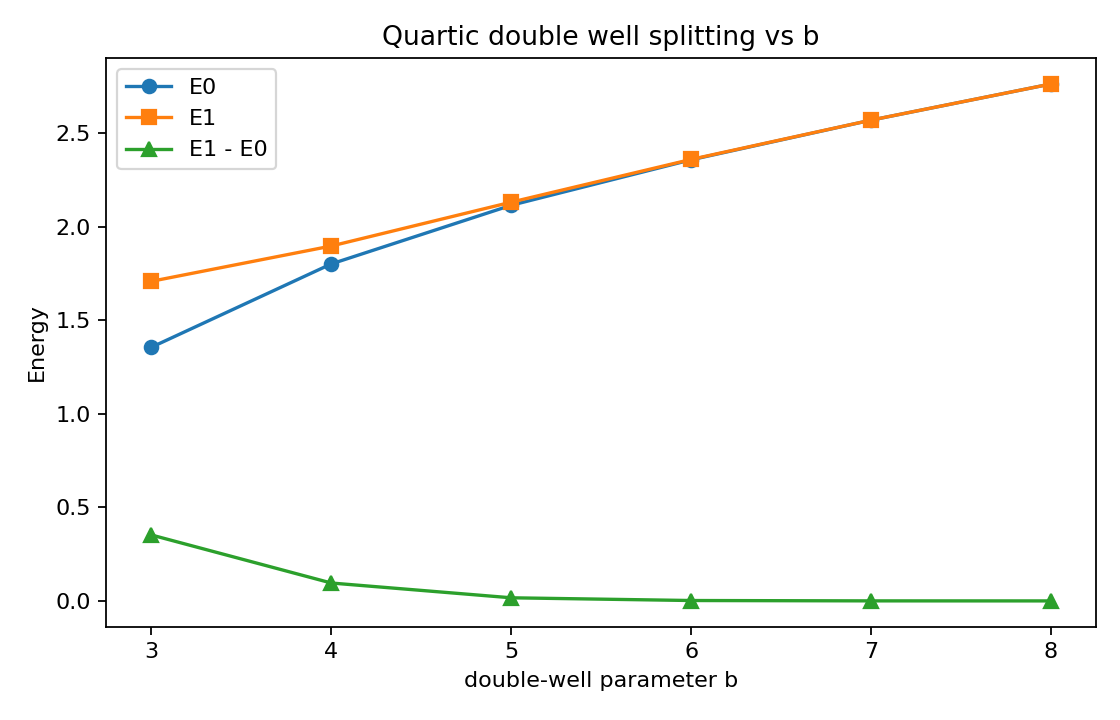
\includegraphics[height=5cm]{../results/3_double_well_Numerov/3_double_well_Numerov_splitting_vs_b.png}
                \caption{Energy splitting between the two lowest double-well states as the parameter $b$ is varied. The splitting decreases as the barrier becomes stronger, consistent with tunneling suppression.}
                \label{fig:dw_splitting}
            \end{figure}

        \subsection{Finite square well}
            The finite square well is included as an additional nontrivial bound-state test. Unlike the infinite square well, the potential walls are finite, so bound states can leak into the classically forbidden region. The potential used here has the form
            \[
            V(x)=\begin{cases}
            0 & |x|\le a,\\
            V_0 & |x|>a,
            \end{cases}
            \]
            and only states with $E<V_0$ are true bound states.

            Figure~\ref{fig:finitewell_states} shows the first four computed states together with the finite well potential. The first three states lie clearly below the barrier and are localized mainly inside the well, with exponentially decaying tails outside. The fourth state is close to the barrier height, and therefore has much stronger leakage into the exterior region. This behavior is physically expected for shallow or near-threshold bound states.

            The probability densities in Fig.~\ref{fig:finitewell_densities} show the same effect more clearly. Low-lying states are concentrated inside the well, while the highest plotted state is spread much farther outside the well. The node count and even-odd structure remain consistent with the ordering of one-dimensional bound states.

            These results are sufficient for the finite square well part of the report because this case is used mainly to demonstrate that the same shooting framework works for a potential with finite barriers and evanescent tails. The more detailed convergence and validation analysis is already provided by the infinite well and harmonic oscillator, while the finite well serves as an additional qualitative and physical test.

            \begin{figure}[!p]
                \centering
                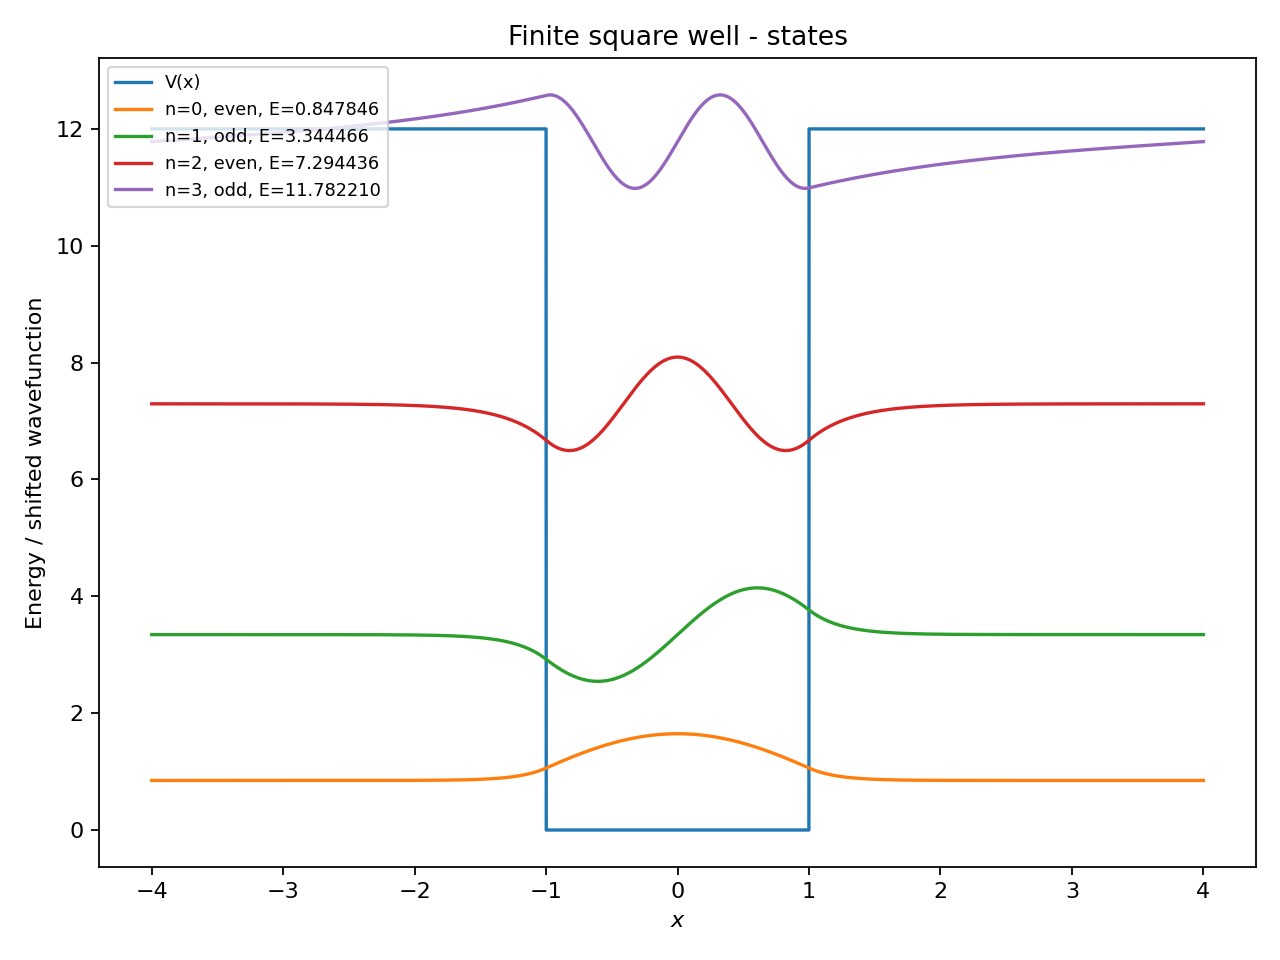
\includegraphics[height=5cm]{../results/4_finite_square_well_Numerov/4_finite_square_well_Numerov_states.png}
                \caption{First four finite square well states plotted together with the finite barrier potential. States below the barrier are localized in the well, while the near-threshold state has a larger evanescent tail.}
                \label{fig:finitewell_states}
            \end{figure}

            \begin{figure}[!p]
                \centering
                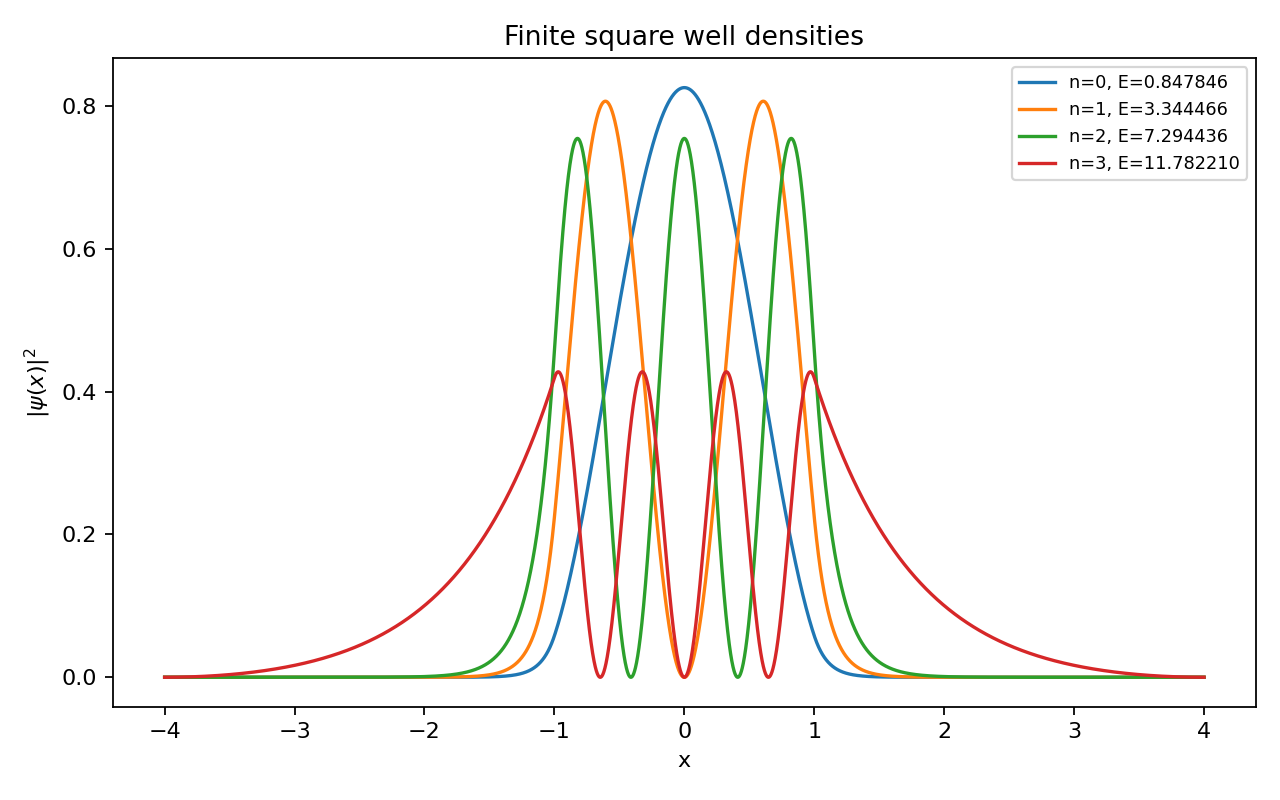
\includegraphics[height=5cm]{../results/4_finite_square_well_Numerov/4_finite_square_well_Numerov_densities.png}
                \caption{Probability densities $|\psi(x)|^2$ for the first four finite square well states. The densities show both interior oscillation and exterior exponential leakage.}
                \label{fig:finitewell_densities}
            \end{figure}

        \subsection{Scattering and resonant tunneling}
            \subsection{Single barrier potential}
                As a secondary extension beyond bound states, the Numerov framework is also applied to one-dimensional scattering from a finite rectangular barrier. For each incident energy $E$, the complex wavefunction is propagated through the barrier region and decomposed into incident, reflected, and transmitted waves. This gives the transmission and reflection probabilities $T(E)$ and $R(E)$.

                The single-barrier result is shown in Fig.~\ref{fig:single_barrier_scattering}. At low incident energy, where $E$ is well below the barrier height, transmission is strongly suppressed and reflection is close to one. As the incident energy increases, the transmission rises smoothly and approaches unity, while reflection decreases. This is the expected qualitative behavior for scattering from a finite barrier.

                The dashed curve shows the conservation check $T(E)+R(E)$, which remains close to one across the full energy range. This confirms that the numerical scattering calculation approximately conserves probability flux. Small deviations near the highest energies are consistent with numerical decomposition and finite-domain effects, and do not affect the qualitative conclusion.

                \begin{figure}[!p]
                    \centering
                    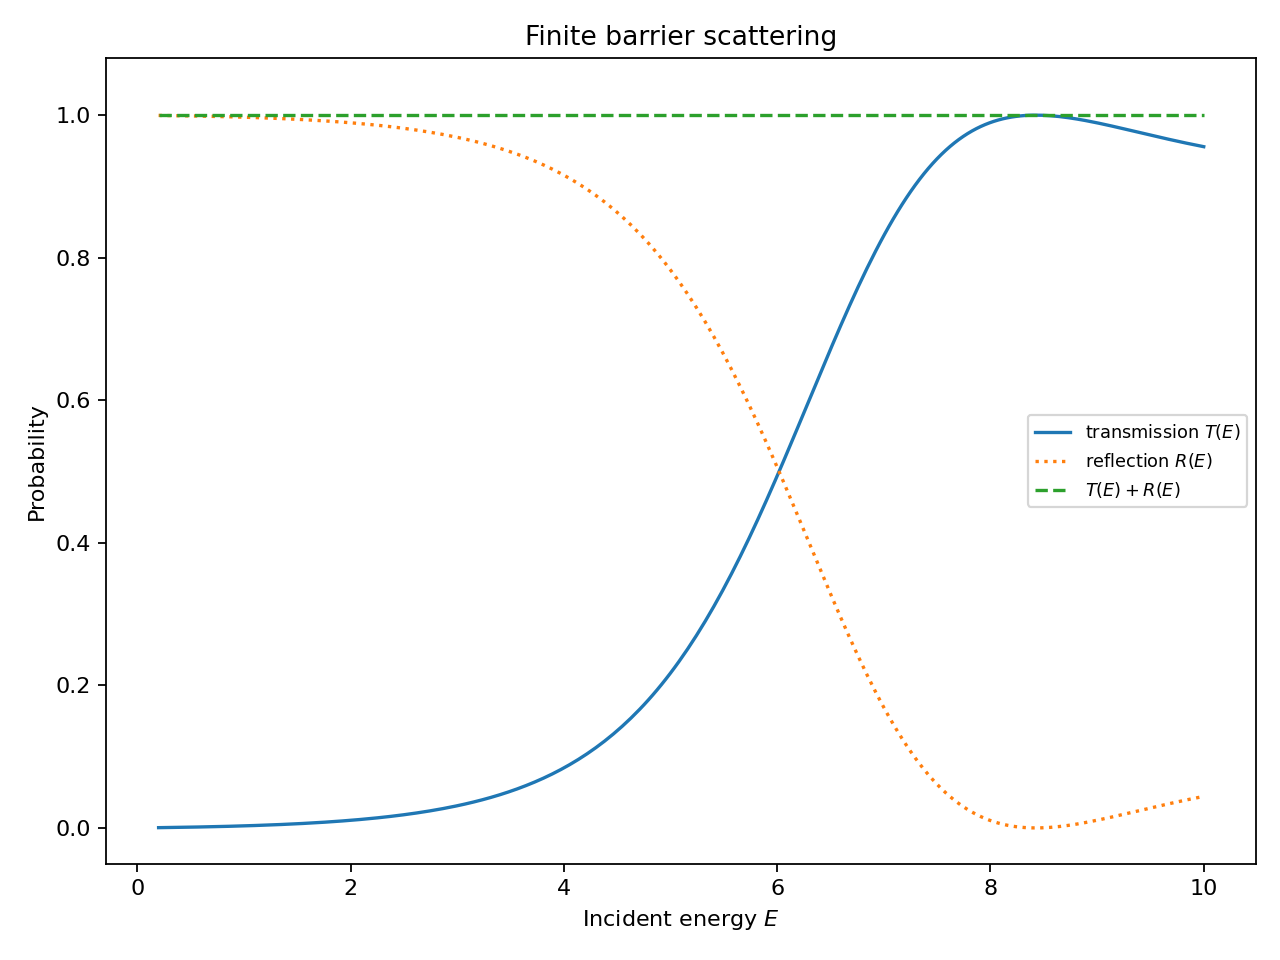
\includegraphics[height=5cm]{../results/5_scattering_single_barrier_Numerov/5_scattering_single_barrier_Numerov_TR.png}
                    \caption{Transmission and reflection probabilities for scattering from a finite rectangular barrier. At low energies reflection dominates, while at high energies transmission approaches unity. The conservation check $T(E)+R(E)$ remains close to one.}
                    \label{fig:single_barrier_scattering}
                \end{figure}

            \subsection{Double barrier potential}
                The double-barrier potential is used to demonstrate resonant tunneling. In this case the two barriers create an intermediate well, so certain incident energies can form quasi-bound states between the barriers. At these energies, destructive reflection and constructive transmission lead to sharp peaks in the transmission coefficient.

                Figure~\ref{fig:double_barrier_resonances} shows the computed transmission and reflection probabilities. The transmission contains a narrow resonance near $E\approx1.139$ and a broader high-energy resonance at larger energy. At the resonant energies, $T(E)$ approaches unity and $R(E)$ drops correspondingly, which is the expected behavior for resonant tunneling through a double barrier.

                The conservation check $T(E)+R(E)$ remains close to one, confirming approximate probability-flux conservation in the scattering calculation. This is an important diagnostic because it verifies that the numerical decomposition into incident, reflected, and transmitted components is self-consistent.

                Figure~\ref{fig:double_barrier_resonant_state} shows the probability density at the first resonance. The wavefunction is strongly enhanced in the region between the two barriers, which is the expected signature of a quasi-bound state. This spatial localization explains the corresponding peak in the transmission spectrum.

                These results are sufficient for the double-barrier part of the report because the scattering section is a secondary extension. The plots demonstrate the key qualitative physics: transmission resonances, reflection suppression at resonance, flux conservation, and enhancement of the wavefunction in the central well.

                \begin{figure}[!p]
                    \centering
                    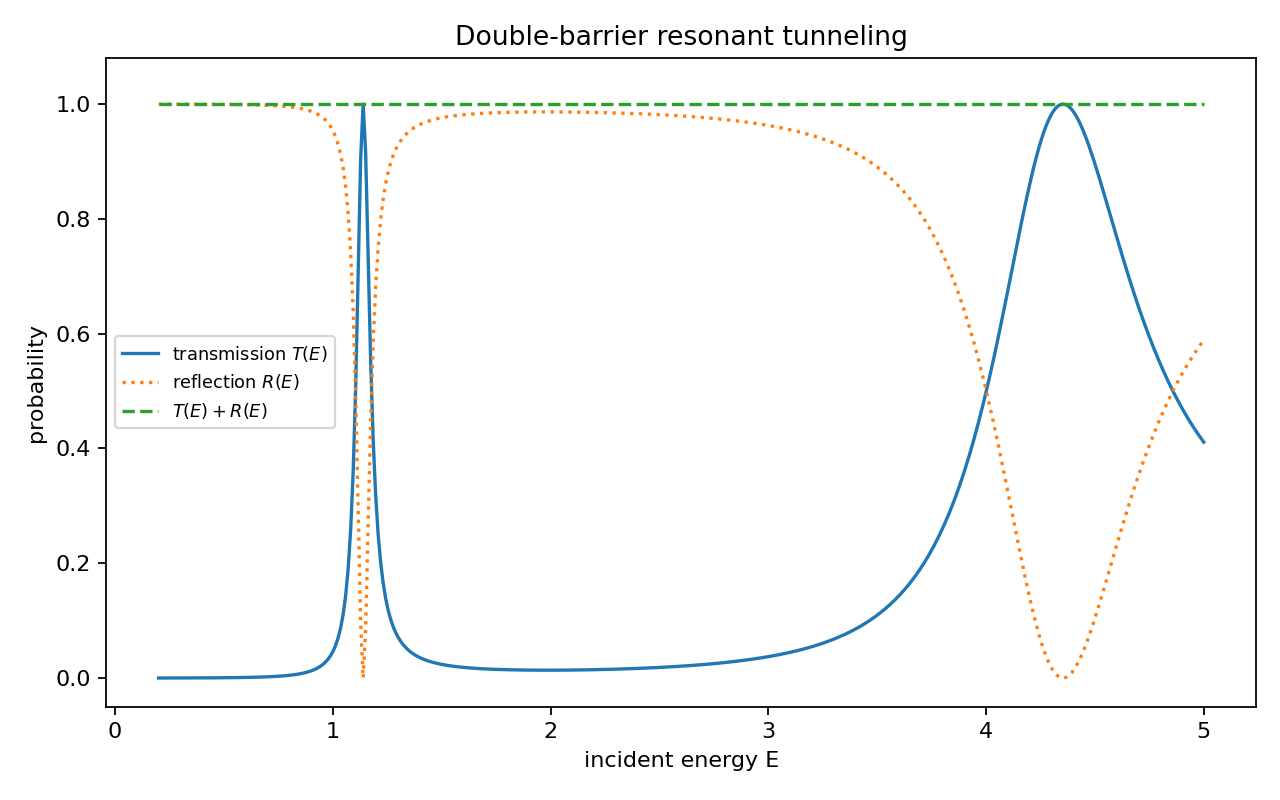
\includegraphics[height=5cm]{../results/6_scattering_double_barrier_Numerov/6_scattering_double_barrier_Numerov_resonances.png}
                    \caption{Transmission and reflection probabilities for the double-barrier potential. Sharp transmission peaks occur at resonant energies, where reflection is suppressed and $T(E)+R(E)$ remains close to one.}
                    \label{fig:double_barrier_resonances}
                \end{figure}

                \begin{figure}[!p]
                    \centering
                    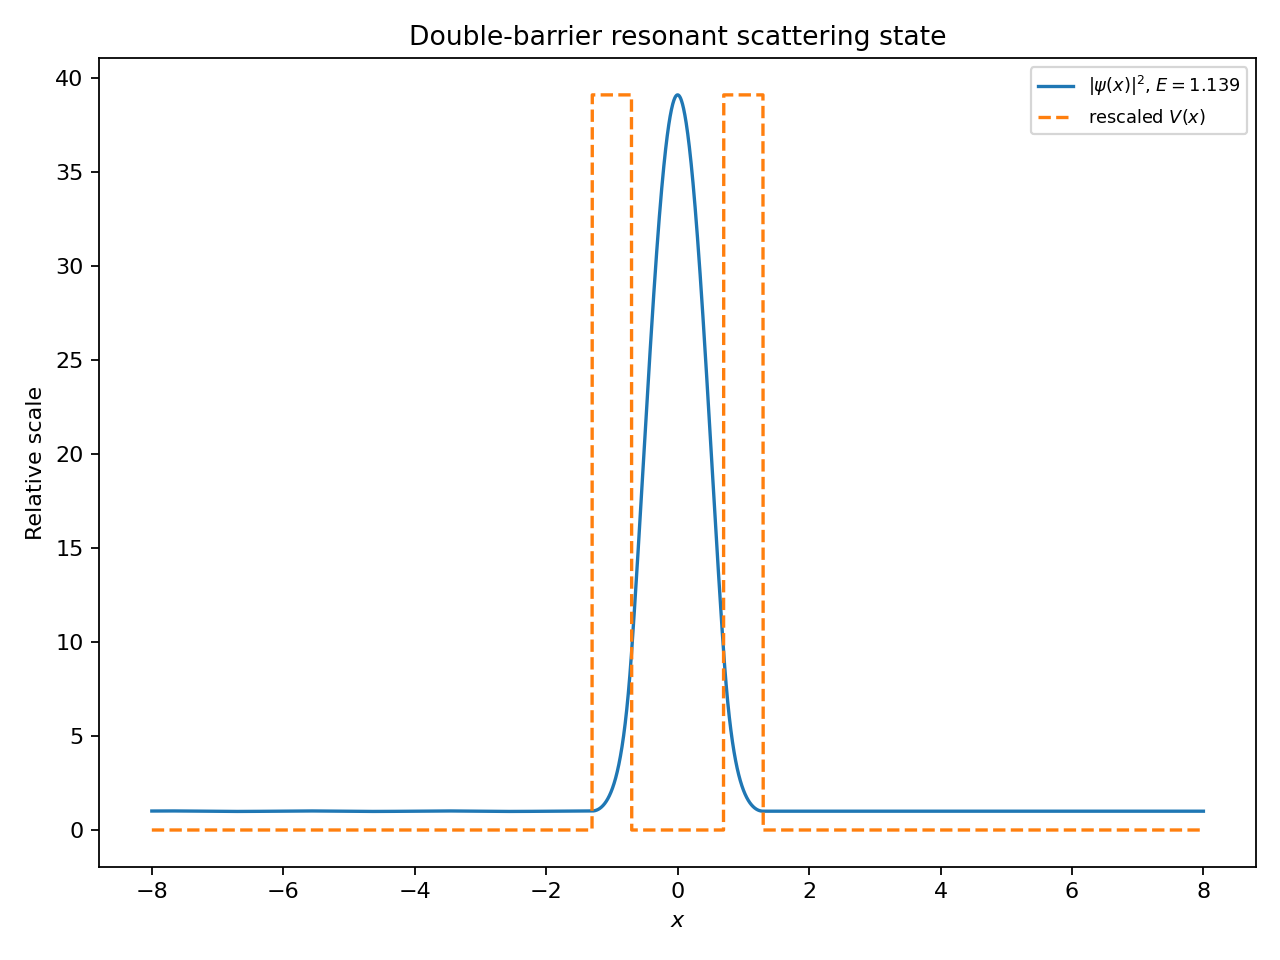
\includegraphics[height=5cm]{../results/6_scattering_double_barrier_Numerov/6_scattering_double_barrier_Numerov_resonant_state.png}
                    \caption{Probability density at the first resonant energy. The wavefunction is strongly enhanced between the two barriers, showing the quasi-bound state responsible for resonant tunneling.}
                    \label{fig:double_barrier_resonant_state}
                \end{figure}

    \subsection{Convergence study}
    We analyze numerical errors by varying both the grid spacing $h$ and the domain size $x_{\max}$.

    \paragraph{Grid convergence.}
    For fixed $x_{\max}$, the energy error follows approximately
    \[
    \Delta E \propto h^p,
    \]
    where $p$ is estimated from log--log fits and reported in the figure legends. The observed values $p\approx 3$--$4$ are consistent with high-order Numerov accuracy, with mild degradation due to boundary truncation and root-finding tolerances.

    \paragraph{Dependence on domain size.}
    For problems on unbounded domains (e.g., the harmonic oscillator), truncation at finite $x_{\max}$ introduces boundary error. For small $x_{\max}$ the wavefunction is artificially cut off, producing large errors. As $x_{\max}$ increases, the error decreases until it reaches a plateau set by discretization, root-finding tolerance, and floating-point precision. Thus this plot measures sensitivity to domain size rather than pure discretization convergence.

    Convergence is primarily established using systems with known analytic solutions (square well and harmonic oscillator), and similar stable behavior is observed for more complex potentials such as the double well, although quantitative error estimates are less accessible there.

    A comparison with a fourth-order Runge--Kutta (RK4) integrator was also performed for the harmonic oscillator. Both methods solve the same shooting problem, but RK4 evolves the wavefunction and its derivative simultaneously, whereas Numerov exploits the specific structure of the Schr\"odinger equation. Initially, RK4 appeared more accurate due to a lower-order derivative approximation in the Numerov boundary condition. After correcting this issue, both methods exhibit comparable convergence behavior, with Numerov achieving similar or better accuracy for the same grid spacing. This highlights the importance of treating boundary conditions with the same order of accuracy as the integration scheme.

    Representative plots include wavefunctions, probability densities, root-finding diagnostics, convergence curves, and energy splitting as a function of potential parameters.

    \section{Discussion}
    The correctness of the code is verified through multiple checks. Analytical benchmarks confirm the accuracy of the computed eigenvalues, while normalization ensures that the wavefunctions remain physically meaningful. Convergence studies provide strong evidence that the numerical results are stable with respect to discretization parameters.

    The double-well analysis highlights a key physical phenomenon: tunneling-induced energy splitting. As the barrier height increases, the splitting decreases, reflecting reduced overlap between the localized states. This demonstrates that the numerical method captures not only correct energies but also meaningful physical behavior.

    The results also illustrate typical numerical considerations, such as sensitivity to grid resolution and domain size, and emphasize the importance of matching the accuracy of boundary conditions to that of the integration scheme.

    The agreement with analytical results, together with consistent convergence behavior and well-behaved root-finding diagnostics, demonstrates the correctness and robustness of the numerical implementation. Differences in observed convergence rates across states are attributed to boundary truncation and solver tolerances rather than defects in the underlying method.

    \section{Conclusion}
    The Numerov method, combined with parity-based shooting and robust root-finding, provides an efficient and accurate tool for one-dimensional bound-state problems, with controlled errors from discretization, domain truncation, and floating-point precision. In addition to reproducing known spectra, it captures physically interesting effects such as tunneling-induced energy splitting in a double well.

    The extension to scattering problems further demonstrates the flexibility of the approach as a secondary component, allowing the study of transmission, reflection, and resonant tunneling phenomena within the same numerical framework.

    \printbibliography[heading=bibintoc,title={References}]
    \end{refsection}

\end{document}
